\documentclass[a4paper,10pt, twocolumn]{article}
\usepackage[a4paper,top=2cm,bottom=3cm,left=2cm,right=2cm,footskip=0.8cm]{geometry}
\usepackage[utf8]{inputenc}
\usepackage{lipsum}
\usepackage{graphicx}
\usepackage{float}
\usepackage{caption}    % Para personalizar legendas, opcionalrefe
\usepackage{xcolor}
\usepackage{fancyhdr}
\usepackage{helvet}
\usepackage{multicol}
\usepackage{titlesec}     % Para personalizar \section
\usepackage[style=ieee, sorting=nty, language=portuguese]{biblatex}
\definecolor{grayFEI}{HTML}{7F7F7F}
\usepackage{paracol} % no preâmbulo
\usepackage{titlesec}
\usepackage{indentfirst}  % Indenta o primeiro parágrafo
\setlength{\parindent}{2em}  % Aumenta a indentação para 2em (pode ser ajustado
\titlespacing*{\section}{0pt}{*0}{0pt}
\usepackage{ragged2e}
\usepackage{multirow}
\usepackage{array}
\usepackage{booktabs}
\usepackage{tikz}
\usepackage{cuted}
\usetikzlibrary{matrix, positioning, arrows.meta, chains, shapes.geometric, calc, fit, backgrounds}
\usepackage{listings}
\usepackage{adjustbox}
\usepackage{hyperref}
\usepackage{graphicx}
\usepackage{float}
\usepackage{multirow}
\usepackage{tabularx}

\definecolor{codegreen}{rgb}{0,0.6,0}
\definecolor{codegray}{rgb}{0.5,0.5,0.5}
\definecolor{codepurple}{rgb}{0.58,0,0.82}
\definecolor{backcolour}{rgb}{0.95,0.95,0.92}

\lstdefinestyle{mystyle}{
    backgroundcolor=\color{backcolour},   
    commentstyle=\color{codegreen},
    keywordstyle=\color{magenta},
    numberstyle=\tiny\color{codegray},
    stringstyle=\color{codepurple},
    basicstyle=\ttfamily\footnotesize,
    breakatwhitespace=false,         
    breaklines=true,                 
    captionpos=b,                    
    keepspaces=true,                 
    numbers=left,                    
    numbersep=5pt,                  
    showspaces=false,                
    showstringspaces=false,
    showtabs=false,                  
    tabsize=2
}


%-------------------------- ESTILOS NÃO ALTERAR ------------------------------------------------%
% Estilo para legendas de figura e tabela
\captionsetup[figure]{
  labelfont={color=azulFEI, bf, small, sf}, % "Figura" azul, negrito, Arial-like
  textfont={small, sf},                    % Texto da legenda em Arial-like
  font=footnotesize,                       % Tamanho aproximado de 9pt
  labelsep=period,                         % "Figura 1." e não "Figura 1:"
  name=Figura,                             % Tradução para "Figura"
  justification=raggedright,              % Alinhado à esquerda
  singlelinecheck=false                   % Garante alinhamento mesmo em uma linha
}

\captionsetup[table]{
  labelfont={color=azulFEI, bf, small, sf},
  textfont={small, sf},
  font=footnotesize,
  labelsep=period,
  name=Tabela,
  justification=raggedright,
  singlelinecheck=false
}

% Formatação section e subsection
\titleformat{\subsection}
  {\color{grayFEI}\normalfont\fontfamily{phv}\selectfont\itshape\fontsize{10}{12}\selectfont}
  {\thesubsection.}{0.2em}{}
\renewcommand{\thesubsection}{\Alph{subsection}}

\titleformat{\section}
  {\color{azulFEI}\normalfont\fontfamily{phv}\selectfont\bfseries\fontsize{11}{13}\selectfont} % Fonte Helvetica, tamanho 11pt, negrito
  {\thesection.}{0.2em}{}
\renewcommand{\thesection}{\Roman{section}} 
\titlespacing*{\section}
{0pt}{10pt}{0pt}

%Formatação Título
\newcommand{\inovatitle}[1]{%
  \noindent{\fontsize{18}{20}{\helvet{\textbf{\textcolor{azulFEI}{#1}}}}}\vspace{25pt}
}

%Formatação Autores
\newcommand{\autores}[1]{
  \helvet{\fontsize{11}{20}\selectfont\textbf{\textit{#1}}}
}
\newcommand{\orientador}[1]{
  \helvet{\fontsize{11}{20}\selectfont\textbf{\textit{#1}}}
}
\newcommand{\filiacao}[1]{
  \helvet{\fontsize{10}{20}\selectfont{\textit{#1}}}
}
\newcommand{\email}[1]{
  \helvet{\fontsize{10}{20}\selectfont{\textit{#1}}\newline}
}
\newcommand{\resumo}[1]{%
\vspace{15pt}
  \noindent
  {\helvet{\fontsize{12}{20}\selectfont\textbf{\textcolor{azulFEI}{Resumo:}}}} %
  \justifying #1 %
  \newline
}

\newcommand{\keyword}[1]{
  \noindent\helvet{\fontsize{12}{20}\selectfont\textbf{\textcolor{azulFEI}{Palavras-chaves:}}} #1  \vspace{25pt}
}

\renewcommand{\thetable}{\Roman{table}}


% Define a cor azul específica (exemplo: azul FEI)
\definecolor{azulFEI}{HTML}{0070C0} % substitua pelo código que quiser

%Formatação Cabeçalho e rodapé
\setlength{\headsep}{1cm}
\newcommand{\helvet}[1]{{\fontfamily{phv}\selectfont #1}}
\pagestyle{fancy}
\fancyhead{} % limpa cabeçalho
\renewcommand{\headrulewidth}{0.3pt} % ← ATIVA a linha (espessura ajustável)
\setlength\headheight{1.2cm}
\lhead{
\includegraphics[width=4.97cm, height=1cm]{logoinovatcc2.png}}
\rhead{\helvet{2º semestre/2026}}

\fancyfoot{} % limpa rodapé
\lfoot{
  \fontfamily{phv}\fontsize{8}{10}\selectfont
  Anais dos Trabalhos de Conclusão de Curso do Centro Universitário FEI, São Bernardo do Campo – SP\\
  \vspace{-4pt}\rule{\textwidth}{1pt} % ← linha abaixo do texto do rodapé
}
\rfoot{\fontfamily{phv}\fontsize{8}{10}\selectfont \thepage}

%-------------------------------- FIM ESTILOS ---------------------------------------------------%



%Adicionar a bibliografia
\addbibresource{referencias.bib}


\begin{document}

\setlength{\columnsep}{20pt}
\twocolumn[
\begin{@twocolumnfalse}

\raggedright

\inovatitle{Tecnologias de Machine Learning para Detecção de Intrusões em Redes de Computadores: Uma Pesquisa Exploratória e Experimental}

\autores{$^1$Lucas Kerr do Amaral, $^2$Marcela Nalesso}

\filiacao{$^1$ Ciência da Computação – FEI}
\filiacao{$^2$ Ciência da Computação – FEI}

\email{$^1$lamaral2002@gmail.com, $^2$marcelanalesso@gmail.com}

\filiacao{Orientador: Prof. Dr. Leonardo Anjoletto Ferreira}
\email{laferreira@fei.edu.br}

\resumo{
	Diante da insuficiência performática dos métodos tradicionais de detecção, 
	este trabalho apresenta o desenvolvimento de um Sistema de Detecção de Intrusão 
	em Redes (NIDS) baseado em Aprendizado de Máquina. Na primeira etapa, 
	realizou-se uma pesquisa exploratória em lote no conjunto de dados NSL-KDD com 
	redução de dimensionalidade (PCA e matriz de correlação de \textit{Pearson}), na qual o 
	algoritmo \textit{Decision Tree} alcançou 99,7\% de acurácia. Em seguida, desenvolveu-se 
	uma arquitetura operacional em tempo real conteinerizada (\textit{Docker} sob Proxmox 
	com \textit{bridge} em \textit{ageing time} zero e interface em modo promíscuo), estruturada em 
	dois estágios de classificação: \textit{Isolation Forest} para detecção de anomalias 
	(integrado a uma \textit{Decision Tree surrogate} para explicabilidade) e SVM Linear 
	para a classificação refinada de ameaças. Como resultados do protótipo, 
	obteve-se um sistema funcional e resiliente ao envenenamento de modelos, capaz 
	de operar de forma contínua, mantendo a taxa de falsos positivos (FPR) $\leq 2\%$ no 
	controle benigno e garantindo a preservação do \textit{recall} por cenário de ataque.
}

\keyword{Sistemas de Detecção de Intrusões, Machine Learning, Segurança da Informação, Análise de Dados, Redução de Dimensionalidade e Cybersegurança.}

\end{@twocolumnfalse}

]
% \twocolumn[
% \begin{@twocolumnfalse}
% \section{Lista de Abreviaturas e Siglas}
\begin{description}
\item[DoS] \textit{Denial of service} ataque que consiste em negar o serviço para outros acessos.
\item[R2L] \textit{Remote to local} escalação de serviço de um acesso remoto para permissão local.
\item[U2R] \textit{User to Root} escalação de privilégios de usuário com baixo nível de permissão para usuário com nível administrativo.
\item[IDS] \textit{Introsion Detection System} Sistema de detecção de intrusão.
\item[HIDS] \textit{Host based Intrusion detection System} Sistemas $IDS$ baseados em host.
\item[NIDS] \textit{Network based Intrusion detection System} Sistemas $IDS$ baseados em tráfego de rede.
\item[Zero-Day] Ataques onde se tem o conhecimento a zero dias (ataques inéditos).
\item[ML] \textit{Machine Learning} algorítimos de aprendizado de máquina.
\item[PCA] \textit{Principal Component Analysis} analise de componentes principais.
\item[SVM] \textit{Support Vector Machine} algorítimo de $ML$ baseado em um vetor de suporte para classificação.
\item[IoT] \textit{Internet of Things} Conceito de integração de sistemas embarcados.
\item[5G] Redes móveis de alta velocidade.
\item[CART] \textit{Classification and Regression Tree} Modelo de arvore de decisão para classificação e regressão.
\item[One-Class SVM] algorítimo de $SVM$ não supervisionado utilizado para detecção de anomalias.
\item[NSL-KDD] Base de dados estudada neste artigo.
\item[ADFA] \textit{Intrusion Detection Systems Dataset}.
\item[ID3] \textit{Iterative Dichotomizer} Algorítimo utilizado para gerar arvores de decisão.
\item[C4.5] Algorítimo utilizado para gerar árvores de decisão, sucessor do $ID3$.
\item[SOM] Mapas auto-organizáveis.
\item[Overfitting] Situação onde a árvore fina desbalanceada.
\item[MultiTree] Algorítmos baseados em multiplas árvores.
\item[REPTree] Algorítmo de árvore de decisão rápida.
\item[stepwise] Método automático de seleção de variáveis preditoras.
\item[Apache Spark] Software para processamento distribuido.
\item[AUROC] Métrica para avaliar desempenho de modelos de classificação binária.
\item[Probe] Ataques de mapeamento de informações sobre o alvo.
\item[StandardScaler] Ferramenta de pré-processamento para padronizar atributos.
\item[Decision Tree] Algorítimo de árvore de decisão.
\item[Random Forest] Algorítimo que cria diversas árvores de decisão e vota entre valores em comum.
\item[KNN] \textit{K Nearest-Neighbor} Método de $ML$ supervisionado para classificação e regressão.
\item[Logistic Regression] Método de $ML$ que calcula a regressão logística dos atributos.
\item[LoadModules] Carregamento de módulos de linguagens como $perl$ para uso indevido.
\item[Perl] Linguagem de programação.
\item[nmap] Software de análise e mapeamento de rede e host.
	
\end{description}

% \end{@twocolumnfalse}
% ]
% \section{Lista de Abreviaturas e Siglas}

\section{Introdução}

% VOU COLOCAR ALGUNS DADOS NESSA INTRODUÇÃO

O avanço das redes de computadores e a crescente digitalização de serviços têm 
ampliado significativamente a exposição de sistemas a ameaças cibernéticas. Esse 
crescimento é acompanhado por um aumento expressivo no volume de dados trafegados, 
que passou de aproximadamente 16 GB por usuário ao mês em 2017 para cerca de 50 GB 
mensais em 2022 \cite{Thakkar2021Survey}. Esse cenário contribui diretamente para a ampliação da superfície 
de ataque, refletindo no aumento da quantidade e da sofisticação de ameaças, como 
negações de serviço, varreduras de rede e acessos não autorizados. Paralelamente, os 
impactos de falhas de segurança tornam-se cada vez mais críticos, sendo que mais de 
14 bilhões de registros de dados foram vazados desde 2013, além de prejuízos 
financeiros significativos, como os 29,8 bilhões de dólares perdidos em golpes 
telefônicos apenas no ano de 2020 \cite{zehedi2023comparative}. Diante desse contexto, a área de Segurança da 
Informação destaca-se como fundamental para garantir a integridade, confidencialidade 
e disponibilidade das informações.

Os Sistemas de Detecção de Intrusão ($IDS$) são fundamentais para a segurança de 
redes, pois monitoram atividades suspeitas e identificam possíveis ataques 
por meio da análise de tráfego e comportamento. Esses sistemas podem ser 
implementados em \textit{hardware} ou \textit{software} e realizam funções como geração de 
alertas e resposta a incidentes. O conceito de IDS surgiu na década de 1980, 
inicialmente baseado na análise de \textit{logs} e padrões conhecidos, o que limitava 
sua eficácia frente a ameaças mais complexas. Com o avanço dos ataques, os 
$IDS$ evoluíram para abordagens mais dinâmicas, incorporando análise comportamental 
e, posteriormente, técnicas de detecção por anomalias na década de 1990, 
permitindo a identificação de ataques desconhecidos \cite{patrick2022study}. Dessa forma, os IDS 
consolidaram-se como mecanismos essenciais para a proteção de ativos digitais 
e mitigação de ameaças em redes \cite{emad2022intrusion}. 

Nesse sentido, o uso de técnicas de Aprendizado de Máquina tem se consolidado como uma 
alternativa promissora \cite{Khraisat2019Survey}. Esses métodos permitem a identificação de padrões complexos 
nos dados, possibilitando a detecção de comportamentos anômalos sem depender 
exclusivamente de regras pré-definidas. No entanto, a eficácia desses modelos 
depende diretamente da qualidade dos dados utilizados, da seleção adequada de 
atributos e da capacidade de lidar com a alta dimensionalidade das bases. Assim, 
compreender a influência dessas variáveis torna-se essencial para o 
desenvolvimento de soluções mais eficientes.

Dessa forma, este trabalho tem como objetivo geral projetar, implementar e avaliar 
um Sistema de Detecção de Intrusão em Redes (NIDS) baseado em Aprendizado de Máquina, 
evoluindo de um estudo exploratório experimental em lote (MVP1) para uma arquitetura 
operacional conteinerizada em tempo real, apta a monitorar o tráfego continuo e 
dotada de mecanismos de defesa contra o envenenamento de modelos (MVP2). Para 
alcançar o objetivo geral, definem-se os seguintes objetivos específicos:

\begin{itemize}
    \item Construir e implantar a infraestrutura de monitoramento em tempo real (MVP2): estruturar uma arquitetura conteinerizada via \textit{Docker Compose} em ambiente virtualizado Proxmox, configurando a interface da máquina virtual em modo promíscuo e a ponte virtual (\textit{bridge}) com tempo de envelhecimento (\textit{ageing time}) ajustado para zero, garantindo a captura não destrutiva e a análise integral do tráfego em trânsito.
    \item Implementar a arquitetura de classificação em dois estágios encadeados: desenvolver o Estágio 1 empregando o algoritmo não supervisionado \textit{Isolation Forest} para filtragem de anomalias em tempo real — acompanhado por uma árvore de decisão substituta \textit{Decision Tree} surrogate para a geração de regras explicativas de alerta — e o Estágio 2 empregando um SVM Linear supervisionado para a classificação detalhada de ameaças conhecidas a partir de vereditos do analista \textit{active learning}.
    \item Estabelecer mecanismos de resiliência ao envenenamento de modelos (\textit{model poisoning}): estruturar um ciclo de vida de treinamento sustentado por um \textit{data pool} curado, aplicando regras operacionais de quarentena de 7 dias, recência temporal com meia-vida de 14 dias e descarte automatizado de janelas identificadas como contaminadas.
	\item Validar a performance e a segurança da esteira de promoção: submeter os modelos candidatos ao teste automatizado frente a um conjunto \textit{benchmark} rotulado (\textit{Golden Set}), utilizando um portão de validação (\textit{validation gate}) que exige a preservação do \textit{recall} por cenário de ataque e impõe o limite de taxa de falsos positivos (FPR $\leq 2\%$) no controle benigno para a efetivação da promoção em produção.
\end{itemize}

Este trabalho está estruturado em cinco capítulos principais. Além desta Introdução, 
o Capítulo 2 apresenta a Fundamentação Teórica sobre arquiteturas de rede, 
sistemas IDS e algoritmos de aprendizado de máquina através de trabalhos relacionados, 
mapeando o estado da arte na literatura. O Capítulo 3 detalha a Metodologia e 
Arquitetura do Sistema, contemplando as fases experimental (MVP1) e operacional em 
tempo real (MVP2). O Capítulo 4 apresenta os Resultados e Discussão, comparando os 
desempenhos em lote e contínuo. Por fim, o Capítulo 5 sintetiza as Conclusões e 
indica diretrizes para trabalhos futuros.

\section{Fundamentação Teórica}

\subsection{Segurança da Informação e Ameaças em Redes de Computadores}
A segurança da informação tornou-se um elemento central na sociedade 
contemporânea devido à crescente dependência de sistemas digitais. Com a 
consolidação da chamada “civilização cibernética” \cite{wasyhun2023cyber}, iniciada a partir da 
revolução digital no final do século XX \cite{Kazi2019network}, houve um aumento significativo na 
produção e circulação de dados, ampliando a superfície de ataque para agentes 
maliciosos. Nesse cenário, a segurança mostra-se indispensável, sobretudo 
pelo uso intensivo de sistemas digitais em setores críticos como bancos, 
saúde, governo e educação, nos quais a proteção das informações é fundamental 
para garantir a continuidade dos serviços, a confiabilidade das operações e a 
segurança da sociedade como um todo \cite{wasyhun2023cyber}.

É desta forma que o foco central da área de pesquisa é proteger dados contra 
ameaças internas e externas, assegurando a tríade CIA (também conhecida como tríade AIC) de confidencialidade (\textit{confidentiality}), 
integridade (\textit{integrity}) e disponibilidade (\textit{availability}) de forma eficiente e com o menor custo 
possível \cite{diptiben2022cyber}. Nesse contexto, evidencia-se que ataques cibernéticos representam 
riscos significativos para as organizações, podendo ocasionar perdas 
financeiras expressivas, danos à reputação institucional e até impactos 
críticos, inclusive fatais, quando afetam infraestruturas essenciais \cite{wasyhun2023cyber}. Além 
disso, observa-se que organizações estão constantemente sob ataques 
direcionados, o que reforça a complexidade e a frequência dessas ameaças no 
ambiente digital contemporâneo \cite{diptiben2022cyber}. Dessa forma, torna-se imprescindível a adoção 
de estratégias robustas de segurança da informação, capazes de mitigar riscos 
e garantir a proteção contínua dos ativos informacionais diante de um cenário 
cada vez mais hostil.

As ameaças em redes de computadores apresentam diversidade e complexidade, 
sendo classificadas em diferentes categorias conforme seu objetivo e forma de 
atuação. Entre as principais estão os ataques de negação de serviço ($DoS$), 
que visam indisponibilizar recursos, ataques de sondagem (\textit{probing}), que 
coletam informações da rede, além de técnicas de escalonamento de privilégios 
($U2R$) e acesso remoto indevido ($R2L$) \cite{wasyhun2023cyber}. Além dessas categorias, destacam-se
ameaças modernas como malware, botnets e ataques de engenharia social, que 
exploram vulnerabilidades técnicas e humanas \cite{Thakkar2021Survey} \cite{solane2015using}. Essa variedade evidencia que os 
sistemas precisam lidar não apenas com ataques diretos, mas também com 
estratégias sofisticadas de invasão e evasão. Portanto, a classificação das 
ameaças é fundamental para orientar mecanismos de detecção e defesa mais 
eficientes. 

Um dos maiores desafios atuais da segurança em redes está relacionado aos 
ataques de $Zero-Day$, que exploram vulnerabilidades ainda desconhecidas pelos 
sistemas de defesa. Por não possuírem assinaturas previamente registradas, 
esses ataques são difíceis de identificar por métodos tradicionais, 
funcionando como ameaças invisíveis até que sejam descobertas \cite{wasyhun2023cyber}. Casos reais, 
como a Operação Aurora, demonstram o potencial destrutivo dessas ameaças, 
incluindo roubo de dados sensíveis e comprometimento de infraestruturas 
críticas \cite{wasyhun2023cyber}. Além disso, o aumento significativo desse tipo de ataque nos últimos 
anos reforça a necessidade de abordagens mais avançadas de detecção. Dessa 
forma, a evolução das ameaças exige a adoção de soluções mais inteligentes e 
adaptativas. 

\subsection{Sistemas de Detecção de Intrusão}
Nesse contexto, os Sistemas de Detecção de Intrusão ($IDS$) desempenham um papel 
central na proteção de redes, sendo responsáveis por monitorar atividades e 
identificar comportamentos suspeitos. Esses sistemas permitem a detecção 
precoce de ataques, possibilitando ações de mitigação antes que danos maiores 
ocorram. No entanto, ainda apresentam limitações importantes, como altas taxas 
de falsos positivos e dificuldade na identificação de ataques desconhecidos \cite{emad2022intrusion}. 
Tais limitações evidenciam a necessidade de evolução desses mecanismos, 
especialmente com o uso de técnicas mais avançadas, como aprendizado de 
máquina, capazes de analisar padrões complexos e melhorar a eficiência da 
detecção \cite{patrick2022study}. Assim, o aprimoramento dos $IDS$ é fundamental para enfrentar os 
desafios contemporâneos da segurança em redes. 

Os $IDS$ podem ser classificados de acordo com sua forma de implantação e método 
de detecção, o que influencia diretamente sua eficiência. Quanto à 
implantação, destacam-se os sistemas baseados em host ($HIDS$), que monitoram 
atividades locais, e os baseados em rede ($NIDS$), que analisam o tráfego em 
pontos estratégicos da infraestrutura. Já em relação ao método de detecção, 
os $IDS$ podem operar por meio de assinaturas, identificando padrões conhecidos 
de ataques, ou por anomalias, detectando desvios em relação ao comportamento 
considerado normal. Além disso, abordagens híbridas combinam essas técnicas 
para superar limitações individuais \cite{Khraisat2019Survey} \cite{zehedi2023comparative} \cite{Thakkar2021Survey} \cite{Khraisat2019Hybrid}. Essa diversidade de classificações 
demonstra a necessidade de adaptar os mecanismos de detecção conforme o 
contexto e os tipos de ameaças enfrentadas. Portanto, a escolha do tipo de $IDS$ 
deve considerar os requisitos específicos do ambiente. 

Apesar de sua relevância, os $IDS$ ainda apresentam limitações significativas 
que comprometem sua eficácia. Sistemas baseados em assinatura, por exemplo, 
são incapazes de identificar ataques desconhecidos, como os de $Zero-Day$, 
enquanto sistemas baseados em anomalias podem gerar altas taxas de falsos 
positivos ao interpretar comportamentos legítimos como ameaças \cite{Kazi2019network}. Além disso, 
muitos $IDS$ enfrentam desafios relacionados ao alto custo computacional, 
datasets mais modernos e à dificuldade de operar em tempo real em ambientes 
com grande volume de tráfego. Essas limitações evidenciam que, embora 
essenciais, os $IDS$ tradicionais ainda não são totalmente suficientes para 
lidar com a complexidade das ameaças modernas \cite{emad2022intrusion} \cite{patrick2022study}. Dessa forma, torna-se 
necessário aprimorar continuamente esses sistemas. 

\subsection{Aprendizado de Máquina em IDS}
O uso de \textit{Machine Learning} ($ML$) tem se consolidado como uma abordagem fundamental 
para aprimorar os Sistemas de Detecção de Intrusão ($IDS$), permitindo a 
análise automatizada de grandes volumes de dados de rede. Diferentemente dos 
métodos tradicionais, o $ML$ possibilita a identificação de padrões complexos e 
a detecção de atividades maliciosas sem a necessidade de intervenção humana 
constante. Isso ocorre porque os modelos são capazes de aprender a partir de 
dados históricos, tornando os sistemas mais adaptativos e eficientes na 
identificação de ameaças \cite{zehedi2023comparative} \cite{Thakkar2021Survey}. Dessa forma, o $ML$ amplia significativamente a 
capacidade dos $IDS$ em lidar com ambientes dinâmicos e com grande volume de 
tráfego. Assim, sua aplicação representa um avanço importante na evolução das 
soluções de segurança de redes. 

As técnicas de \textit{Machine Learning} aplicadas aos $IDS$ podem ser classificadas em 
diferentes abordagens, sendo as mais comuns o aprendizado supervisionado, não 
supervisionado e por reforço. Além disso, o 
processo de construção desses modelos envolve a divisão dos dados em conjuntos 
de treinamento e teste, garantindo a avaliação do desempenho do sistema \cite{zehedi2023comparative} \cite{emad2022intrusion}. Essa 
diversidade de abordagens permite que os $IDS$ sejam adaptados a diferentes 
cenários e tipos de ataque, aumentando sua flexibilidade e eficiência. 
Portanto, a escolha da técnica de aprendizado influencia diretamente a 
eficácia da detecção de intrusões. 

Entre os principais benefícios do uso de $ML$ em $IDS$ está a capacidade de 
detectar ataques desconhecidos, como os $Zero-Day$, além de lidar com relações 
complexas e não lineares presentes nos dados de rede \cite{zehedi2023comparative} \cite{Kazi2019network}. No entanto, essa 
abordagem também apresenta desafios relevantes, como o alto custo 
computacional e o tempo elevado de treinamento. Outro problema recorrente é o 
desbalanceamento dos dados, que dificulta a detecção de ataques menos 
frequentes, impactando negativamente o desempenho dos modelos. Essas 
limitações evidenciam que, embora o $ML$ traga avanços significativos, sua 
aplicação ainda exige cuidados na preparação e tratamento dos dados \cite{zehedi2023comparative}. Dessa 
forma, o sucesso do uso de $ML$ em $IDS$ depende não apenas dos algoritmos, mas 
também da qualidade dos dados utilizados. 

Além disso, etapas como pré-processamento, seleção de atributos e redução de 
dimensionalidade são essenciais para garantir o desempenho dos modelos de 
\textit{Machine Learning} em $IDS$. A limpeza dos dados, normalização e codificação de 
variáveis contribuem para a construção de modelos mais robustos, enquanto 
técnicas como seleção de atributos e métodos como $PCA$ ajudam a reduzir a 
complexidade dos dados e melhorar a acurácia. Para avaliar a eficácia dos 
modelos, são utilizadas métricas como acurácia, precisão, \textit{recall} e \textit{F1-score}, 
que permitem analisar o equilíbrio entre a detecção de ataques e a geração de 
falsos positivos. Assim, a integração entre boas práticas de tratamento de 
dados e algoritmos de $ML$ é fundamental para o desenvolvimento de $IDS$ mais 
eficientes e confiáveis \cite{zehedi2023comparative} \cite{Thakkar2021Survey}. Portanto, o uso estruturado dessas técnicas 
potencializa os resultados obtidos na detecção de intrusões. 

A diversidade de algoritmos utilizados em sistemas de detecção de intrusão é 
destacada em \cite{Liao2013Intrusion}, que realiza uma revisão 
abrangente das técnicas de $IDS$, incluindo métodos baseados em Bayes, teoria 
dos jogos e mineração de dados. O estudo evidencia que algoritmos de 
mineração, como árvores de decisão, e métodos como $SVM$ apresentam altas taxas 
de acurácia na detecção de ataques. Esses resultados indicam que não existe 
uma abordagem única dominante, mas sim um conjunto de técnicas complementares 
que podem ser utilizadas conforme o contexto da aplicação.	

\subsection{Trabalhos Relacionados}
Liao et al.\cite{Liao2013Intrusion} revisam técnicas de IDS baseadas em Bayes, teoria dos jogos 
e mineração de dados, e mostram que árvores de decisão e SVM apresentam altas 
taxas de acurácia, sem uma abordagem dominante. Saranya et al. \cite{Saranya2020Performance} comparam 
algoritmos em cenários IoT e 5G e obtêm 99,65\% de acurácia com Random Forest, 
contra 98\% do CART isolado. Khraisat et al. \cite{Khraisat2019Hybrid} combinam C5.0 e One-Class SVM 
em um modelo híbrido, com 83,24\% de acurácia no NSL-KDD e 97,04\% no ADFA, mostrando 
que a combinação entre detecção por assinatura e por anomalia supera as limitações 
individuais — ideia próxima da cascata adotada no MVP2.

A interpretabilidade das árvores de decisão é destacada por Azam et al. \cite{zehedi2023comparative}, em que o CART alcançou 
97,36\% de sucesso. Depren et al. \cite{Depren2005Intelligent} combinam C4.5 com mapas auto-organizáveis (SOM) e atingem 
99,84\% na detecção de uso indevido. Gao et al. \cite{Xianwei2019Adaptive} propõem o MultiTree, um ensemble de árvores CART 
com votação majoritária que trata o desbalanceamento e alcança 85,2\% em cenários desafiadores. 
Rathore et al. \cite{Rathore2016RealTime} usam C4.5 e REPTree em ambiente de Big Data com apenas 9 atributos e obtêm taxa de 
verdadeiros positivos acima de 99,9\%. Abdulganiyu et al. \cite{Abdulganiyu2023Systematic} consolidam que algoritmos baseados em 
árvores variam entre 85,2\% e 99,9\% de acurácia, conforme a preparação dos dados.

Quanto ao pré-processamento, Vanin et al. \cite{patrick2022study} destacam o alto número de atributos 
do KDDCup99 (41) e do CICIDS2017 (80) e a necessidade de técnicas como o PCA. Thakkar e Lohiya \cite{Thakkar2021Survey} 
mostram que reduzir para 5 a 20 atributos relevantes melhora a eficiência dos algoritmos. 
Iglesias e Zseby \cite{felix2014analysis} reduzem de 41 para 16 atributos sem perda de acurácia, e Othman et al. \cite{Othman2018Intrusion} 
selecionam 17 atributos por quiquadrado e obtêm AUROC de 99,55\%. Abdallah et al. \cite{emad2022intrusion} reforçam que 
conjuntos de 10 a 19 atributos são comuns em abordagens eficientes. 

\subsection{Isolation Forest}
O Isolation Forest \cite{Tony2008Isolation} detecta anomalias isolando pontos em vez de modelar a densidade do normal. 
Cada árvore particiona os dados com cortes aleatórios até isolar cada amostra; pontos raros e distantes 
são isolados com poucos cortes. O \textit{score} de anomalia de uma amostra x em um conjunto de n amostras é 
\begin{equation}
s(x, n) = 2^{-\frac{E[h(x)]}{c(n)}},
\end{equation}
em que E[h(x)] é a profundidade média de isolamento de x nas árvores e c(n) é a profundidade média 
de uma busca malsucedida em árvore binária, usada como normalização. Escores próximos de 1 indicam 
anomalia. O parâmetro contamination define a fração de amostras de treino marcadas como anômalas e, 
portanto, o limiar de decisão. Uma consequência estrutural explorada na Seção IV, é que um conjunto 
volumoso e homogêneo de amostras de ataque deixa de ser raro e passa a ser difícil de isolar.

\subsection{Máquinas de Vetores de Suporte}
A SVM \cite{Corinna1995Support} procura o hiperplano $f(x) = w^\top x + b$ de máxima margem entre duas classes. Na versão 
linear, o valor de f(x) é uma distância com sinal ao hiperplano (a menos do fator $\|w\|$): o sinal dá 
a classe predita e o módulo dá a confiança. Essa propriedade é usada no Estágio 2 para ordenar a 
fila de revisão do analista. Por ser supervisionada, a SVM só reconhece formas de ataque que já viu 
rotuladas.

\subsection{Envenamento de Modelos e Aprendizado Ativo}
Ataques de envenenamento (\textit{poisoning}) manipulam os dados de treino para degradar ou desviar um modelo \cite{Battista2012Poisoning}. 
Em um IDS que se retreina sobre o tráfego observado, o atacante não precisa injetar dados artificialmente: 
basta que sua própria atividade, mantida em volume baixo e regular, entre no conjunto de treino e passe a 
ser aprendida como normal. 
O aprendizado ativo (\textit{active learning}) \cite{Settles2009Active} reduz o custo de rotulagem escolhendo 
quais amostras submeter ao especialista. A estratégia por incerteza prioriza as amostras mais próximas da 
fronteira de decisão, nas quais um rótulo humano mais altera o modelo. 

\subsection{NSL-KDD e CIC-IDS2017}
A adoção do conjunto de dados NSL-KDD é fundamental para garantir a padronização dos testes e a comparabilidade científica 
do modelo de detecção de intrusões, evitando os vieses estatísticos inerentes às bases legadas. Conforme detalhado no 
artigo de revisão de Thakkar e Lohiya \cite{Thakkar2021Survey}, o NSL-KDD foi desenvolvido a partir do clássico KDD Cup '99 especificamente para 
solucionar falhas estruturais graves, eliminando aproximadamente 78\% das instâncias duplicadas presentes no conjunto de 
treinamento e 75\% no conjunto de testes. A remoção desse elevado volume de dados redundantes previne que os algoritmos 
de Machine Learning fiquem tendenciosos em relação a padrões de tráfego normal frequentes, permitindo um aprendizado mais 
justo sobre categorias de ataques raros e danosos, como \textit{User-to-Root} (U2R) e \textit{Remote-to-Local} (R2L)\cite{Thakkar2021Survey}.

Por outro lado, a utilização da base de dados CIC-IDS2017 justifica-se pela imperiosa necessidade de validar o modelo proposto 
perante um ambiente de tráfego de rede contemporâneo e altamente diversificado. De acordo com o estudo sistemático de 
Abdulganiyu et al. \cite{Abdulganiyu2023Systematic} e o levantamento de Thakkar e Lohiya \cite{Thakkar2021Survey}, o dataset CIC-IDS2017, criado pelo \textit{Canadian Institute 
for Cybersecurity}, disponibiliza 80 características extraídas de fluxos de rede \textit{pcap} e contempla uma vasta gama de 
ameaças modernas, tais como \textit{DoS-Hulk}, \textit{Botnets}, \textit{Brute Force} (SSH/FTP), \textit{PortScan} e \textit{Heartbleed} \cite{Abdulganiyu2023Systematic} \cite{Thakkar2021Survey}. Enquanto datasets legados 
falham em refletir os comportamentos do tráfego web atual, o CIC-IDS2017 fornece perfis realistas obtidos de uma topologia de rede 
completa e interações com múltiplos sistemas operacionais e tráfego criptografado\cite{Abdulganiyu2023Systematic} \cite{Thakkar2021Survey}. 

A fim de organizar e comparar os principais trabalhos\footnote{Arquivo disponível em: \url{https://1drv.ms/x/c/46f377637be54264/IQB7NxizkmLAS7_X22no62qJAZll5FV9_5Dt7G3kALLXvTY?e=ypAxe1}} relacionados à detecção 
de intrusões e machine learning, foi elaborada a Tabela XI encontrada na seção de Anexos contendo os 
estudos mais relevantes identificados na literatura. 
%VERIFICAR O NÚMERO DA TABELA PRA ANEXAR NESSA PARTE DEPOIS

%A tabela apresenta 
%critérios como tipo de abordagem, técnicas utilizadas e bases de dados 
%empregadas, permitindo uma análise comparativa entre as propostas.

%\footnote{\url{https://www.unb.ca/cic/datasets/kdd.html}}.
%ESTOU TESTANDO O ESTILO E SE A TABELA VAI FICAR LEGAL ASSIM


\section{Metodologia}

% Este trabalho propõe uma abordagem voltada na avaliação do desempenho de algoritmos 
% de aprendizado de máquina não supervisionados aplicados à detecção de intrusões em redes 
% de computadores. A metodologia adotada foi estruturada em etapas sequenciais, 
% contemplando desde a seleção das bases de dados até a avaliação dos algoritmos 
% utilizados, conforme ilustrado na Figura \ref{fig:metodologia}.

A pesquisa possui caráter aplicado, com abordagem quantitativa, objetivo 
experimental e busca comparar o desempenho de diferentes algoritmos de 
classificação a partir da utilização de técnicas de redução e seleção de atributos. O sistema é desenvolvido em $python$ e implementado em $Docker$.
O fluxo metodológico foi dividido em cinco etapas principais: seleção das bases de 
dados, processamento dos dados, aplicação de técnicas de redução de dimensionalidade, 
treinamento dos algoritmos e avaliação de desempenho. seguido pela implementação do MVP2 em um pipeline de dois algorítimos que utilizam $Isolation Forest$ + $Decision Tree$ (estágio 1) e $SVM$ linear (estágio 2) \ref{fig:fases}\\
Todo o código foi estruturado em $python$ utilizando as bibliotecas do \textit{scikit-learn} \cite{scikit2026learn}, $Pandas$ e $scapy$/$nfstream$ para a leitura de pacotes em disco, e conteinerizado em $Docker$ \cite{Merkel2014Docker}.

\begin{figure}[H]
	\centering
	% Visão geral das duas fases do trabalho (coluna simples)
\resizebox{\columnwidth}{!}{%
\begin{tikzpicture}[
  node distance=0.35cm and 0.45cm,
  every node/.style={font=\scriptsize},
  block/.style={rectangle, draw, rounded corners=1pt, text width=1.75cm,
                align=center, minimum height=0.85cm, inner sep=2pt},
  fase/.style={draw=azulFEI, dashed, rounded corners=3pt, inner sep=5pt},
  rot/.style={font=\scriptsize\bfseries\sffamily, text=azulFEI},
  arrow/.style={-{Stealth[length=4pt]}}
]
  % MVP1
  \node (nsl)   [block] {Base NSL-KDD};
  \node (pre)   [block, right=of nsl] {Pré-processa\-mento};
  \node (red)   [block, right=of pre] {Correlação, PCA e importância};
  \node (alg)   [block, right=of red] {5 algoritmos supervisio\-nados};
  \node (av)    [block, right=of alg] {Validação + KDDTest+};

  \foreach \a/\b in {nsl/pre, pre/red, red/alg, alg/av} \draw[arrow] (\a) -- (\b);

  % MVP2
  \node (pcap)  [block, below=1.25cm of nsl] {Tráfego espelhado (pcap)};
  \node (feat)  [block, right=of pcap] {17 atributos por fluxo};
  \node (e1)    [block, right=of feat] {Estágio 1: \textit{Isolation Forest} + árvore};
  \node (e2)    [block, right=of e1] {Estágio 2: SVM linear};
  \node (an)    [block, right=of e2] {Analista: veredito};

  \foreach \a/\b in {pcap/feat, feat/e1, e1/e2, e2/an} \draw[arrow] (\a) -- (\b);
  \draw[arrow] (an.south) -- ++(0,-0.3) -| node[pos=0.25, below]{rótulos} (e2.south);

  \coordinate (anbaixo) at ([yshift=-0.45cm]an.south);
  \begin{scope}[on background layer]
    \node[fase, fit=(nsl)(av)] (f1) {};
    \node[fase, fit=(pcap)(an)(anbaixo)] (f2) {};
  \end{scope}
  \node[rot, anchor=south west] at (f1.north west) {MVP1 --- fluxo metodológico};
  \node[rot, anchor=south west] at (f2.north west) {MVP2 --- operação em tempo real};

  \path (f2.north) coordinate (f2topo);
  \draw[arrow, gray, dashed] (av.south) -- (av.south |- f2topo)
     node[midway, right, text width=2.1cm, align=left] {lacuna de generalização};
\end{tikzpicture}%
}

	\caption{Fases de estudo/implementação do projeto}
	\label{fig:fases}
\end{figure}

\subsection{MVP1}
\subsubsection{Seleção das Bases de Dados}
A base de dados utilizada neste trabalho foi a $NSL-KDD$, uma versão aprimorada da 
base KDD Cup 1999, desenvolvida com o objetivo de reduzir redundâncias e 
inconsistências presentes no conjunto original. A escolha dessa base ocorreu devido 
à sua ampla utilização na literatura científica voltada à detecção de intrusões e 
aprendizado de máquina, sendo considerada uma das principais referências para 
avaliação de sistemas $IDS$. A base contém registros de 
conexões de rede classificados entre tráfego normal (53,46\%) e diferentes categorias 
de ataques (46,54\%), possibilitando a aplicação de técnicas de classificação 
supervisionada.

Os dados foram obtidos por meio da plataforma \textit{Kaggle}\footnote{Disponível em: \url{https://www.kaggle.com/datasets/hassan06/nslkdd}}, utilizando a biblioteca 
\textit{KaggleHub}. Os métodos e técnicas testadas estão disponíveis em \cite{scikit2026learn}, pois foram utilizadas na implementação 
das técnicas de aprendizado de máquina, incluindo codificação de atributos categóricos, 
padronização dos dados, aplicação do $PCA$, divisão dos conjuntos de treinamento e 
teste, treinamento dos algoritmos e validação dos modelos. Essas ferramentas foram 
fundamentais para o processamento dos dados e análise dos resultados obtidos ao 
longo da pesquisa.

\subsubsection{Processamento dos Dados}
Após o carregamento da base de dados $NSL-KDD$, foi realizada uma etapa de 
pré-processamento com o objetivo de preparar os dados para aplicação dos 
algoritmos de aprendizado de máquina. Inicialmente, foram definidos manualmente 
os nomes dos 41 atributos da base, permitindo melhor interpretação das variáveis 
e facilitando a manipulação das informações durante o desenvolvimento do projeto. 
Em seguida, os dados foram carregados em estruturas do tipo \textit{DataFrame} utilizando 
a biblioteca \textit{Pandas}, possibilitando operações de análise, filtragem e 
transformação dos registros. Durante essa etapa, também foi realizada a 
verificação da estrutura da base, incluindo quantidade de linhas, colunas, 
tipos de dados e identificação das classes presentes no conjunto de dados. A 
coluna \textit{label} foi convertida em binário, classificando como 0 para tráfego normal 
e 1 para qualquer tipo de ataque ($DoS$, $Probe$, $R2L$, $U2R$). Posteriormente, a 
coluna denominada \textit{difficulty} foi removida, por ser considerada irrelevante para 
o processo de classificação e não contribuir significativamente para o desempenho 
dos modelos.

% Aqui é legal colocar alguma referência de texto? Tem textos que usaram a mesma base e tem essas descrições...

Na sequência, foi realizada uma análise exploratória dos atributos categóricos 
presentes na base, especialmente nas colunas relacionadas ao protocolo de rede 
(\textit{protocol\_type}), serviço (\textit{service}) e status da conexão (\textit{flag}). Foram analisados 
os valores únicos de cada atributo, permitindo compreender melhor a distribuição 
das informações presentes na base. Como algoritmos de aprendizado de máquina 
supervisionado trabalham predominantemente com dados numéricos, foi necessário 
converter os atributos categóricos para representações numéricas. Para isso, foi 
utilizada a técnica de \textit{Label Encoding}, disponibilizada pela biblioteca \textit{Scikit-learn}, 
responsável por transformar cada categoria textual em um valor inteiro 
correspondente. Essa etapa foi fundamental para garantir a compatibilidade dos 
dados com os algoritmos utilizados posteriormente no treinamento dos modelos.

Além da transformação dos atributos categóricos, também foi realizado um processo 
de agrupamento das classes originais de ataques presentes na base $NSL-KDD$. 
Inicialmente, a base possui diversos tipos específicos de ataques, o que poderia 
aumentar a complexidade do problema de classificação. Dessa forma, os ataques 
foram reorganizados em categorias mais abrangentes, sendo elas \cite{Belavagi2016Performance} \cite{Jabez2015Intrusion}: 
\begin{itemize}
	\item \textbf{Normal:} Tráfego legítimo e sem atividades maliciosas.
	\item \textbf{DoS (Denial of Service):} Ataques que visam sobrecarregar os recursos do sistema, tornando-o indisponível para usuários legítimos.
	\item \textbf{Probe:} Ataques de sondagem que buscam coletar informações sobre o sistema ou rede, identificando vulnerabilidades.
	\item \textbf{R2L (Remote to Local):} Ataques onde o invasor tenta obter acesso local a partir de uma máquina remota, explorando falhas de autenticação.
	\item \textbf{U2R (User to Root):} Ataques onde o invasor já possui acesso local e busca elevar seus privilégios para obter controle total do sistema.
\end{itemize}
Esse agrupamento teve como objetivo simplificar o processo de classificação, 
reduzir a complexidade do problema e melhorar a interpretação dos resultados 
obtidos pelos algoritmos de aprendizado de máquina.

\subsubsection{Redução de Dimensionalidade}
Após a etapa de pré-processamento dos dados, foi realizada uma análise exploratória 
com o objetivo de compreender a estrutura da base $NSL-KDD$, identificar padrões 
nos dados e verificar o comportamento das classes presentes no conjunto 
utilizado. Inicialmente, foram analisadas as dimensões da base de dados, os 
tipos de atributos existentes e a distribuição das classes de ataques. Essa 
etapa permitiu compreender a proporção entre registros classificados como 
tráfego normal e tráfego malicioso, além de identificar possíveis desbalanceamentos 
entre as categorias de ataques. Também foram geradas estatísticas descritivas 
dos atributos numéricos, permitindo observar medidas como média, desvio padrão, 
valores mínimos e máximos das variáveis presentes na base.

Posteriormente, foi aplicada 
uma análise de correlação entre os atributos numéricos da base utilizando o 
coeficiente de correlação de \textit{Pearson}. Essa análise teve como principal objetivo 
identificar relações lineares entre as variáveis e detectar atributos altamente 
correlacionados, que poderiam representar informações redundantes no conjunto 
de dados. 

Com o objetivo de reduzir a dimensionalidade da base e minimizar o impacto do 
elevado número de atributos no desempenho computacional dos modelos, foi 
aplicada a técnica de Análise de Componentes Principais ($PCA$). Antes da 
aplicação do $PCA$, os dados foram padronizados utilizando o método \textit{$StandardScaler$}, 
responsável por transformar os atributos para média igual a zero e desvio padrão 
igual a um. Essa etapa foi necessária porque o $PCA$ é sensível à escala dos dados, 
podendo atribuir maior relevância a atributos com amplitudes maiores. Após a 
padronização, o $PCA$ foi aplicado para transformar os atributos originais em um 
novo conjunto de componentes principais, preservando a maior parte da variância 
existente nos dados. 

Durante essa etapa, foi realizada a análise da variância explicada acumulada dos 
componentes principais, permitindo identificar a quantidade ideal de componentes 
necessários para representar adequadamente o conjunto de dados sem perda 
significativa de informação. 

Por fim, também foi realizada uma etapa de seleção de atributos utilizando o 
algoritmo \textit{$Decision Tree$}. O modelo foi empregado para calcular o grau de importância 
de cada variável durante o processo de classificação, permitindo identificar os 
atributos mais relevantes para o problema de detecção de intrusões. Com base nesses 
resultados, foi possível analisar quais características da base possuíam maior 
influência no desempenho dos modelos de aprendizado de máquina. Essa etapa 
contribuiu para redução de redundâncias, simplificação do conjunto de dados e 
melhoria do desempenho computacional dos algoritmos utilizados posteriormente 
no treinamento e avaliação dos modelos.

\subsubsection{Treinamento dos Algoritmos}
Nessa seção, foi realizada a etapa de treinamento dos algoritmos de aprendizado 
de máquina supervisionado. Essa fase teve como principal objetivo construir 
modelos capazes de identificar padrões presentes nos registros da base $NSL-KDD$ 
e realizar a classificação do tráfego de rede entre conexões normais e 
diferentes categorias de ataques cibernéticos.

Inicialmente, os dados foram organizados em variáveis preditoras (\textit{features}) e 
variável alvo (\textit{target}). Os atributos da base foram utilizados como entrada dos 
algoritmos, enquanto as categorias correspondentes aos tipos de tráfego e 
ataques foram utilizadas como saída esperada dos modelos. Após essa definição, 
os dados passaram pela etapa de separação entre conjuntos de treinamento e teste 
utilizando a função \texttt{train\_test\_split} da biblioteca \texttt{Scikit-learn}, sendo o arquivo 
\texttt{KDDTrain.txt} para treino e o \texttt{KDDTest.txt} para teste, divididos na proporção 
clássica de 70\% e 30\%.  Essa divisão permitiu utilizar parte dos registros 
para treinamento dos algoritmos e outra parte para validação do desempenho dos 
modelos em dados não utilizados durante o aprendizado. Essa abordagem foi 
fundamental para avaliar a capacidade de generalização dos algoritmos e reduzir 
problemas relacionados ao sobreajuste (\textit{$overfitting$}).

Durante os experimentos, foram realizados treinamentos utilizando tanto o 
conjunto completo de atributos quanto versões reduzidas dos dados obtidas por 
meio da aplicação do $PCA$ e da seleção de atributos baseada em importância das 
variáveis. Essa estratégia permitiu comparar o impacto da redução de 
dimensionalidade no desempenho dos modelos, bem como analisar possíveis 
melhorias relacionadas ao custo computacional e à eficiência das classificações. 
Os algoritmos avaliados no treinamento foram: 

\begin{table}[H]
\centering
\footnotesize
\renewcommand{\arraystretch}{0.9}
\setlength{\tabcolsep}{2pt}

\begin{tabularx}{\linewidth}{
>{\hsize=0.45\hsize}X
>{\hsize=0.3\hsize}X
>{\hsize=0.3\hsize}X
>{\hsize=0.3\hsize}X
}
\toprule
\textbf{Algoritmo} & 
\textbf{Tipo} \cite{IBM2026Supervised} & 
\textbf{Definição} \cite{IBM2026Supervised} & 
\textbf{Motivação} \\
\midrule

$Decision Tree$ & 
Aprendizado Supervisionado (Classificação) & 
Cria regras lógicas (fluxograma) para dividir os dados e decidir. & 
Alta interpretabilidade, baixo custo computacional, bom para regras binárias. \\
\\

Random Forest & 
Aprendizado Supervisionado  & 
Combina múltiplas árvores de decisão para previsões mais precisas. & 
Robustez e alta acurácia, porém maior custo. \\
\\

KNN (k=5) & 
Aprendizado Supervisionado (Proximidade) & 
Classifica baseando-se nos vizinhos mais próximos. & 
Simples, útil como baseline não paramétrico. \\
\\

Logistic Regression & 
Aprendizado Supervisionado (Classificação Binária) & 
Calcula a probabilidade de eventos (0\% a 100\%). & 
\textit{Baseline} clássico, rápido e interpretável. \\
\\

SVM (kernel linear) & 
Aprendizado Supervisionado (Classificação) & 
Define o hiperplano que melhor separa grupos de dados. & 
Eficaz em alta dimensionalidade, porém mais lento. \\

\bottomrule
\end{tabularx}

\caption{Comparação de Algoritmos de Aprendizado de Máquina}
\end{table}

Durante o treinamento, os algoritmos aprenderam padrões existentes nos registros 
da base $NSL-KDD$, relacionando características do tráfego de rede às categorias 
de ataques previamente definidas. Os modelos foram ajustados utilizando os dados 
previamente padronizados e transformados, garantindo maior estabilidade durante 
o processo de aprendizado. Além disso, foram realizados testes comparativos 
entre os modelos treinados com os atributos originais e os modelos treinados 
após aplicação das técnicas de redução e seleção de atributos, permitindo analisar 
os impactos dessas abordagens no desempenho final dos classificadores.

Para aumentar a confiabilidade dos resultados obtidos, também foi aplicada a 
técnica de validação cruzada (\textit{cross-validation}). Dessa forma, foi 
possível obter uma avaliação mais consistente e menos dependente de uma única 
divisão aleatória entre treino e teste.

Além das métricas de classificação, também foram analisados aspectos relacionados 
ao desempenho computacional dos modelos, como tempo de treinamento e eficiência 
do processamento após aplicação das técnicas de redução de dimensionalidade. 
Essa análise permitiu verificar não apenas a capacidade dos algoritmos em 
detectar ataques, mas também sua viabilidade computacional para utilização em 
sistemas de detecção de intrusão, nos quais rapidez e eficiência são fatores 
relevantes para o monitoramento do tráfego de rede.

\subsubsection{Avaliação de Desempenho}
Após a etapa de treinamento dos algoritmos de aprendizado de máquina, foi 
realizada a avaliação dos modelos com o objetivo de medir a eficiência dos 
classificadores na detecção de intrusões presentes na base $NSL-KDD$. Durante os 
testes, foram comparados os resultados obtidos pelos modelos treinados com os 
atributos originais da base de dados, pelos modelos treinados após aplicação da 
técnica de redução de dimensionalidade $PCA$ e pelos modelos treinados utilizando 
atributos selecionados com base na importância das variáveis calculadas pelo 
algoritmo \textit{$Decision Tree$}. Essa comparação permitiu analisar o impacto das técnicas 
de redução e seleção de atributos tanto no desempenho dos classificadores 
quanto na eficiência computacional do processamento. 

Para análise dos resultados, foram utilizadas métricas amplamente empregadas em 
problemas de classificação supervisionada e sistemas de detecção de intrusão, 
incluindo \textit{Accuracy}, \textit{Precision}, \textit{Recall} e \textit{F1-Score}. 

Durante a avaliação, também foram observados aspectos relacionados ao desempenho 
computacional dos modelos, incluindo tempo de treinamento, tempo de execução e 
impacto causado pela redução de dimensionalidade no processamento dos dados. 
Essa análise permitiu verificar se a aplicação das técnicas de $PCA$ e seleção de 
atributos contribuiu para redução do custo computacional sem comprometer 
significativamente o desempenho dos classificadores. 

Com base nos resultados obtidos, foi realizada uma comparação entre os algoritmos 
utilizados considerando métricas de desempenho, capacidade de generalização e 
eficiência computacional. O algoritmo \textit{$Decision Tree$} apresentou boa interpretabilidade 
e capacidade de classificação, além de possibilitar a identificação dos 
atributos mais relevantes para o problema. Entretanto, o \textit{$Random Forest$} demonstrou maior 
robustez e estabilidade nas previsões, devido à combinação de múltiplas 
árvores de decisão. A seleção do modelo final considerou o equilíbrio entre as 
métricas de \textit{Accuracy}, \textit{Precision}, \textit{Recall} e \textit{F1-Score}, além do impacto das técnicas de 
redução de dimensionalidade no desempenho e no custo computacional dos algoritmos, 
permitindo identificar a abordagem mais eficiente para classificação do tráfego 
de rede e detecção de intrusões utilizando a base $NSL-KDD$. 

\subsection{MPV2}
O MVP2 é um NIDS que observa uma cópia passiva do tráfego e classifica cada fluxo
em uma cascata de dois modelos (Figura \ref{fig:arquitetura}). Os componentes de
\textit{software} desenvolvidos são:
\begin{itemize}
	\item \textbf{netanomaly.py}: extração de atributos, treino do estágio 1 e métricas e rotulagem das bases.
	\item \textbf{netanomaly\_live.py}: analisador em tempo real, que aplica o modelo congelado a jalenas de 10s.
	\item \textbf{sink.py}: persistência, que grava janelas no \textit{pool} de treino e alertas no banco.
	\item \textbf{lifecycle.py}: ciclo de vida do estágio 1 (\textit{pool}, candidato, portão, promoção, despejo, adoção).
	\item \textbf{netclassify.py}: estágio 2 (veredito, treino, avaliação, promoção predição e fila de revisão).
	\item \textbf{migrations/}: esquema PostgreSQL/TimescaleDB, versionado por migração.
\end{itemize}

\begin{strip}
\begin{figure}[H]
  \centering
  \resizebox{\textwidth}{!}{% Arquitetura do MVP2 (largura total da página).
% Três faixas: detecção (cima), ciclo de vida do Estágio 1 (meio),
% refinamento supervisionado (baixo).
\begin{tikzpicture}[
  every node/.style={font=\scriptsize},
  proc/.style={rectangle, draw, rounded corners=2pt, fill=azulFEI!8,
               text width=2.5cm, align=center, minimum height=1.0cm, inner sep=2pt},
  dado/.style={cylinder, shape border rotate=90, aspect=0.18, draw, fill=gray!10,
               text width=2.4cm, align=center, minimum height=1.0cm, inner sep=1pt},
  ator/.style={rectangle, draw, thick, text width=2.3cm, align=center,
               minimum height=0.9cm, inner sep=2pt},
  zona/.style={draw=gray, dashed, rounded corners=4pt, inner sep=7pt},
  rot/.style={font=\scriptsize\sffamily\bfseries, text=gray},
  arrow/.style={-{Stealth[length=4pt]}},
  lbl/.style={font=\tiny, fill=white, inner sep=1pt}
]
  % ---------------- faixa 1: detecção em tempo real (y = 0)
  \node (span)   [ator] at (0,0)    {Porta espelho (SPAN) ou \textit{bridge}};
  \node (det)    [proc] at (3.4,0)  {$netanomaly\_live$\\extração de fluxos\\(janela de 10 s)};
  \node (e1)     [proc] at (6.8,0)  {\textbf{Estágio 1}\\\textit{Isolation Forest}\\+ árvore \textit{surrogate}};
  \node (sink)   [proc] at (10.2,0) {$sink.py$\\percentil contra a grade do treino};
  \node (alerts) [dado] at (13.6,0) {$na.alerts$\\(\textit{hypertable})};

  % ---------------- faixa 2: ciclo de vida do Estágio 1 (y = -2.9)
  \node (pool)   [dado] at (10.2,-2.9) {\textit{Pool} de \textit{parquets} + $feature\_windows$};
  \node (cand)   [proc] at (6.8,-2.9)  {$lifecycle$\\$candidate$\\(diário, automático)};
  \node (gate)   [proc] at (3.4,-2.9)  {Portão por cenário\\($v\_gate\_verdict$)};
  \node (prom)   [ator] at (0,-2.9)    {Promoção manual\\(troca atômica)};
  \node (gold)   [dado] at (3.4,-4.5)  {\textit{Golden set}\\(cenários rotulados)};

  % ---------------- faixa 3: refinamento supervisionado (y = -6.6)
  \node (e2)     [proc] at (13.6,-6.6) {\textbf{Estágio 2}\\SVM linear\\($netclassify$)};
  \node (fila)   [dado] at (10.2,-6.6) {Predições e fila por margem};
  \node (ana)    [ator] at (6.8,-6.6)  {Analista\\(painel Grafana)};
  \node (ver)    [dado] at (3.4,-6.6)  {$na.verdicts$};
  \node (final)  [dado] at (0,-6.6)    {Classificação final consolidada};

  % setas: detecção
  \draw[arrow] (span) -- (det);
  \draw[arrow] (det) -- (e1);
  \draw[arrow] (e1) -- node[lbl, above=2pt]{escore} (sink);
  \draw[arrow] (sink) -- node[lbl, above=2pt]{$p \geq 0{,}95$} (alerts);

  % setas: ciclo de vida
  \draw[arrow] (sink) -- node[lbl, right=2pt, align=left]{janelas de\\13 min} (pool);
  \draw[arrow] (pool) -- node[lbl, below=15pt, align=center]{quarentena 7 d\\meia-vida 14 d} (cand);
  \draw[arrow] (cand) -- (gate);
  \draw[arrow] (gold) -- (gate);
  \draw[arrow] (gate) -- node[lbl, above=2pt]{aprovado} (prom);
  \draw[arrow] (prom.north) -- ++(0,0.75) -| node[lbl, pos=0.3, above]{novo \texttt{current\_flow.joblib}} (e1.south);

  % setas: refinamento
  \draw[arrow] (alerts) -- node[lbl, right=2pt]{alertas} (e2);
  \draw[arrow] (e2) -- (fila);
  \draw[arrow] (fila) -- node[lbl, above=10pt]{menor margem} (ana);
  \draw[arrow] (ana) -- node[lbl, above=2pt]{veredito} (ver);
  \draw[arrow] (ver.south) -- ++(0,-0.55) -| node[lbl, pos=0.25, below]{rótulos para retreino} (e2.south);
  \draw[arrow] (ver) -- (final);
  \draw[arrow] (fila.north) -- ++(0,0.55) -| node[lbl, pos=0.25, above]{predição (sem veredito)} (final.north);

  \begin{scope}[on background layer]
    \node[zona, fit=(span)(alerts)] (z1) {};
    \node[zona, fit=(prom)(pool)(gold)] (z2) {};
    \node[zona, fit=(final)(e2)] (z3) {};
  \end{scope}
  \node[rot, anchor=south east] at (z1.north east) {detecção em tempo real};
  \node[rot, anchor=south east] at (z2.south east) {ciclo de vida do Estágio 1};
  \node[rot, anchor=north west] at (z3.south west) {refinamento supervisionado};
\end{tikzpicture}
}
  \caption{Arquitetura do MVP2: detecção em tempo real, ciclo de vida do modelo do Estágio 1. refinamento supervisionado do estágio 2.}
  \label{fig:arquitetura}
\end{figure}
\end{strip}

\subsubsection{Ambiente da infraestrutura e conteinerização}

Uma única imagem (\texttt{python:3.13-slim}) serve aos papéis de detector e treinador, garantindo a mesma versão de \textit{scikit-learn} em todos, necessário, pois o artefato \texttt{.joblib} é serializado por versão.
Os containers rodam em \textit{userspace} as capacidades \texttt{cap\_net\_raw} e \texttt{cap\_net\_admin} são
atribuídas ao binário \texttt{tcpdump} como \textit{file capabilities}, de modo que um
processo de UID 1000 abre o \textit{socket} de captura e os arquivos gravados no
volume pertencem ao usuário do hospedeiro. A Tabela \ref{tab:servicos} resume os
serviços do \textit{Docker Compose}; os que capturam ou exibem dados só sobem quando
o perfil correspondente é ativado.

\begin{table}[H]
\centering
\footnotesize
\setlength{\tabcolsep}{3pt}
\begin{tabularx}{\columnwidth}{l l X}
\toprule
\textbf{Serviço} & \textbf{Perfil} & \textbf{Função} \\
\midrule
banco            & ---              & TimescaleDB, porta só em \texttt{127.0.0.1} \\
treinador        & ---              & Migrações, candidato diário e predição do Estágio 2 \\
detector         & sensor           & Captura em \texttt{network\_mode: host} \\
detector-isolado & sensor-isolado   & NIC dedicada via \textit{macvlan passthru} \\
replay           & replay           & Reprocessa um \textit{pcap}, sem captura \\
grafana          & painel           & Painéis dos Estágios 1, 2 e resultado final (consolidado dos estágios anteriores) \\
\bottomrule
\end{tabularx}
\caption{Serviços do \textit{Docker Compose} e perfis de ativação.}
\label{tab:servicos}
\end{table}

\textbf{Persistência.} O banco é PostgreSQL 17 com a extensão TimescaleDB,
organizado no esquema \texttt{na} (14 tabelas e 11 consultas). Quatro
decisões estruturam o esquema:\\ (i) os fluxos ficam em arquivos \textit{Parquet} em disco, e o banco guarda apenas o índice (\texttt{feature\_windows}), com estado de quarentena e despejo;\\ (ii) o corte do
analista é aplicado na consulta, com dois limiares distintos: o
piso de gravação (percentil 0,95, fixo) e o corte de exibição (0,99, ajustável em
uma \textit{view}, com efeito retroativo sem reprocessamento);\\ (iii) \textit{score} contínuo e
percentil são guardados juntos, o primeiro para o Estágio 2 e o segundo para revisão do 
analista;\\ (iv) não há chave estrangeira para a tabela de alertas, pois trata-se de uma
\textit{hypertable} com retenção de 180 dias. Os parâmetros operacionais ficam em uma
tabela editável com histórico de alterações por gatilho. Cada migração é
aplicadas uma única vez por um controlador próprio; se houver falha, o treinador aborta, pois treinar contra um
esquema incerto corromperia a análise.

\textbf{Visualização.} Os painéis do Grafana leem diretamente o banco e cobrem o
Estágio 1 (alertas acima do corte, quase-acertos, janelas no \textit{pool}, portão do
último candidato), o Estágio 2 (dispersão do SVM em PCA 2D, desempenho por cenário,
fila por margem) e o resultado final consolidado. A arquitetura prevista para o
\textit{front-end} é adaptável: parâmetros editados por um painel de formulários do
próprio Grafana.

\subsubsection{Mecanismos de captura e extração de fluxos de rede}

\textbf{Captura.} Um contêiner só enxerga o tráfego que chega ao seu
\textit{namespace} de rede. Por isso o \textit{macvlan} em modo \textit{bridge}. As opções válidas são o modo \textit{host}, em
que o detector vê uma interface promíscua ligada à porta espelho (SPAN) da
\textit{bridge}, e o \textit{macvlan passthru}, que entrega a placa inteira ao contêiner
mantendo-o na rede interna do banco. O arranjo recomendado usa duas interfaces:
uma de gerência, com IP, e uma de captura, sem IP e em modo promíscuo. No
laboratório, a máquina virtual do sensor roda sobre Proxmox, com a interface em
modo promíscuo e a \textit{bridge} virtual com \textit{ageing time} zero, o que faz a
\textit{bridge} repassar todos os quadros a todas as portas, funcionando como um \textit{hub}.
O perfil \texttt{replay} reprocessa um \texttt{pcap} gravado pelo mesmo caminho de
código, o que permite testar o sistema sem captura.

\textbf{Extração.} Os atributos do $NSL-KDD$ não podem ser reproduzidos a partir de
um \textit{pcap} arbitrário: vários dependem de inspeção de conteúdo e de contadores
internos do sensor original. O $MVP2$ define, portanto, seu próprio vetor,
calculável diretamente dos cabeçalhos. Do $MVP1$ vieram a ordem de grandeza (17
atributos) e a evidência de que volume, contagem e taxa de erro de conexão são os
sinais mais discriminantes. Os pacotes são lidos em \textit{streaming}, com memória
proporcional ao número de fluxos, e agregados em duas
visões (Tabela \ref{tab:atributos}) por: fluxo, 5-tupla bidirecional, 
\textit{host} e IP de origem, para capturar o leque de conexões (\textit{fan-out})
típico de varreduras. A visão por fluxo foi a exercitada de ponta a ponta.

\begin{table}[H]
\centering
\footnotesize
\setlength{\tabcolsep}{3pt}
\begin{tabularx}{\columnwidth}{l X}
\toprule
\textbf{Grupo} & \textbf{Atributos} \\
\midrule
\multicolumn{2}{l}{\textbf{Visão por fluxo (17)}} \\
Volume      & \texttt{n\_packets}, \texttt{n\_bytes}, \texttt{duration}, \texttt{bytes\_per\_sec}, \texttt{pkts\_per\_sec} \\
Tamanho     & \texttt{mean\_len}, \texttt{std\_len}, \texttt{min\_len}, \texttt{max\_len} \\
Tempo       & \texttt{mean\_iat}, \texttt{std\_iat} (intervalo entre pacotes) \\
Flags TCP   & \texttt{syn\_ratio}, \texttt{ack\_ratio}, \texttt{fin\_ratio}, \texttt{rst\_ratio}, \texttt{psh\_ratio}, \texttt{syn\_no\_ack} \\
\midrule
\multicolumn{2}{l}{\textbf{Visão por host de origem (11)}} \\
Leque       & \texttt{n\_dst}, \texttt{n\_dports}, \texttt{dports\_per\_dst}, \texttt{pkts\_per\_dst} \\
Volume      & \texttt{h\_packets}, \texttt{h\_bytes}, \texttt{h\_pkts\_per\_sec} \\
Handshake   & \texttt{h\_syn\_ratio}, \texttt{h\_ack\_ratio}, \texttt{h\_rst\_ratio}, \texttt{syn\_ack\_gap} \\
\bottomrule
\end{tabularx}
\caption{Vetores de atributos do MVP2.}
\label{tab:atributos}
\end{table}

\textbf{Duas cadências.} O analisador ao vivo trabalha em janelas de 10~s, que
definem a latência do alerta. O \texttt{sink}, por sua vez, agrupa os fluxos em
janelas de 840s (14min), que são a unidade de treino, quarentena e despejo.

\subsubsection{Arquitetura de Aprendizado em Dois Estágios}
A cascata combina um modelo não supervisionado e um supervisionado. O Estágio 1 não
pode ser supervisionado porque não existe rótulo no tráfego de produção; ele
funciona como peneira, com \textit{recall} alto e precisão baixa. O Estágio 2 opera
apenas sobre os alertas do Estágio 1 e usa rótulos do \textit{golden set} e dos
vereditos do analista, com dois objetivos: recuperar formas de ataque conhecidas
que o Estágio 1 não enxerga e separar ataque real de anomalia benigna.

\textbf{Estágio 1 --- detector não supervisionado.} O detector é um
\texttt{StandardScaler} seguido de um \texttt{IsolationForest} com 200 árvores, ambos
ajustados com pesos por amostra iguais ao peso de recência da janela de origem. O \textit{score} é invertido para que valores maiores signifiquem mais anomalia, e o limiar $\tau$ é o quantil ponderado do \textit{score}
de treino:

\begin{equation}
  s(x) = -\,\mathrm{score}(x), \qquad
  \tau = Q_w\!\left(1 - c\right),
  \label{eq:limiar}
\end{equation}

\noindent em que $c$ é o \textit{contamination} (0,01 por padrão) e $Q_w$ é o quantil
calculado sobre a distribuição acumulada ponderada pelos pesos $w$. O limiar é congelado no artefato: o analisador ao vivo não o recalcula, para que a taxa de alerta não dependa da composição da
janela corrente.

Junto ao limiar, o artefato guarda uma grade de 1.001 quantis do \textit{score} de treino,
e o percentil de cada fluxo é calculado contra essa grade, o “1\% mais anômalo” é tráfego normal.
Contra a grade do treino, uma janela tranquila não gera alerta, e o percentil fica
disponível imediatamente.

Para a explicabilidade, uma \texttt{DecisionTreeClassifier} de profundidade 4 é
treinada sobre os atributos não escalados, tendo como alvo o rótulo atribuído
pelo próprio \textit{Isolation Forest} (Figura \ref{fig:arvore}). A regra do caminho
percorrido por cada alerta (por exemplo, \texttt{n\_bytes <= 143452 e bytes\_per\_sec > 3273625 e ack\_ratio <= 0,932})
é exibida ao analista em unidades reconhecíveis (Figura \ref{fig:janela_analista}.
\begin{figure}[H]
  \centering
  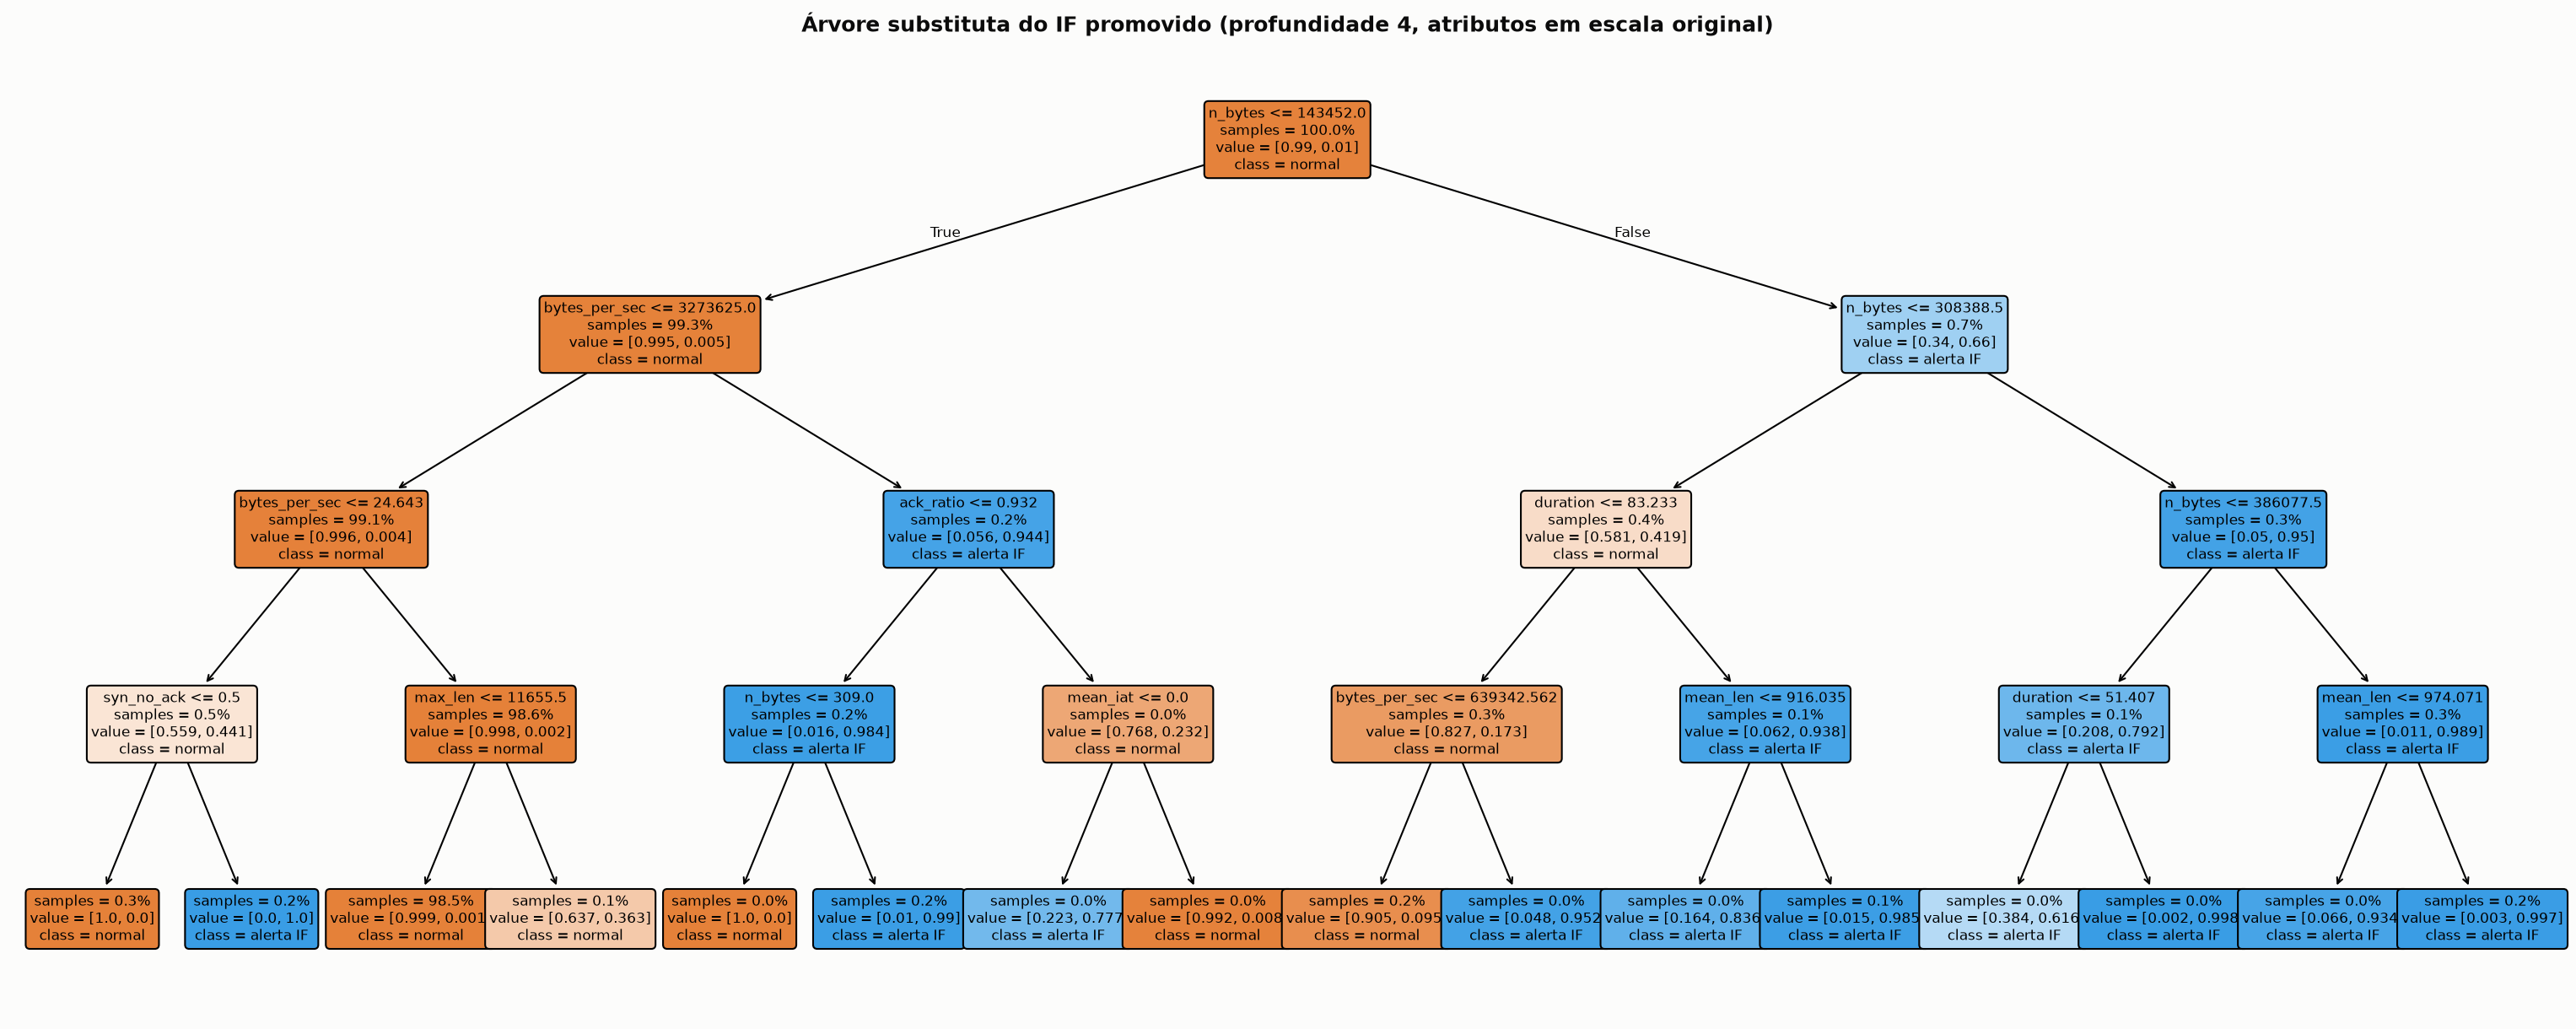
\includegraphics[width=\linewidth]{../../notebooks/figuras/B2_arvore.png}
  \caption{Árvore \textit{surrogate} do \textit{Isolation Forest} promovido (profundidade 4, atributos em escala original). Em laranja, folhas classificadas como normais; em azul, como alerta.}
  \label{fig:arvore}
\end{figure}
\begin{figure}[H]
  \centering
  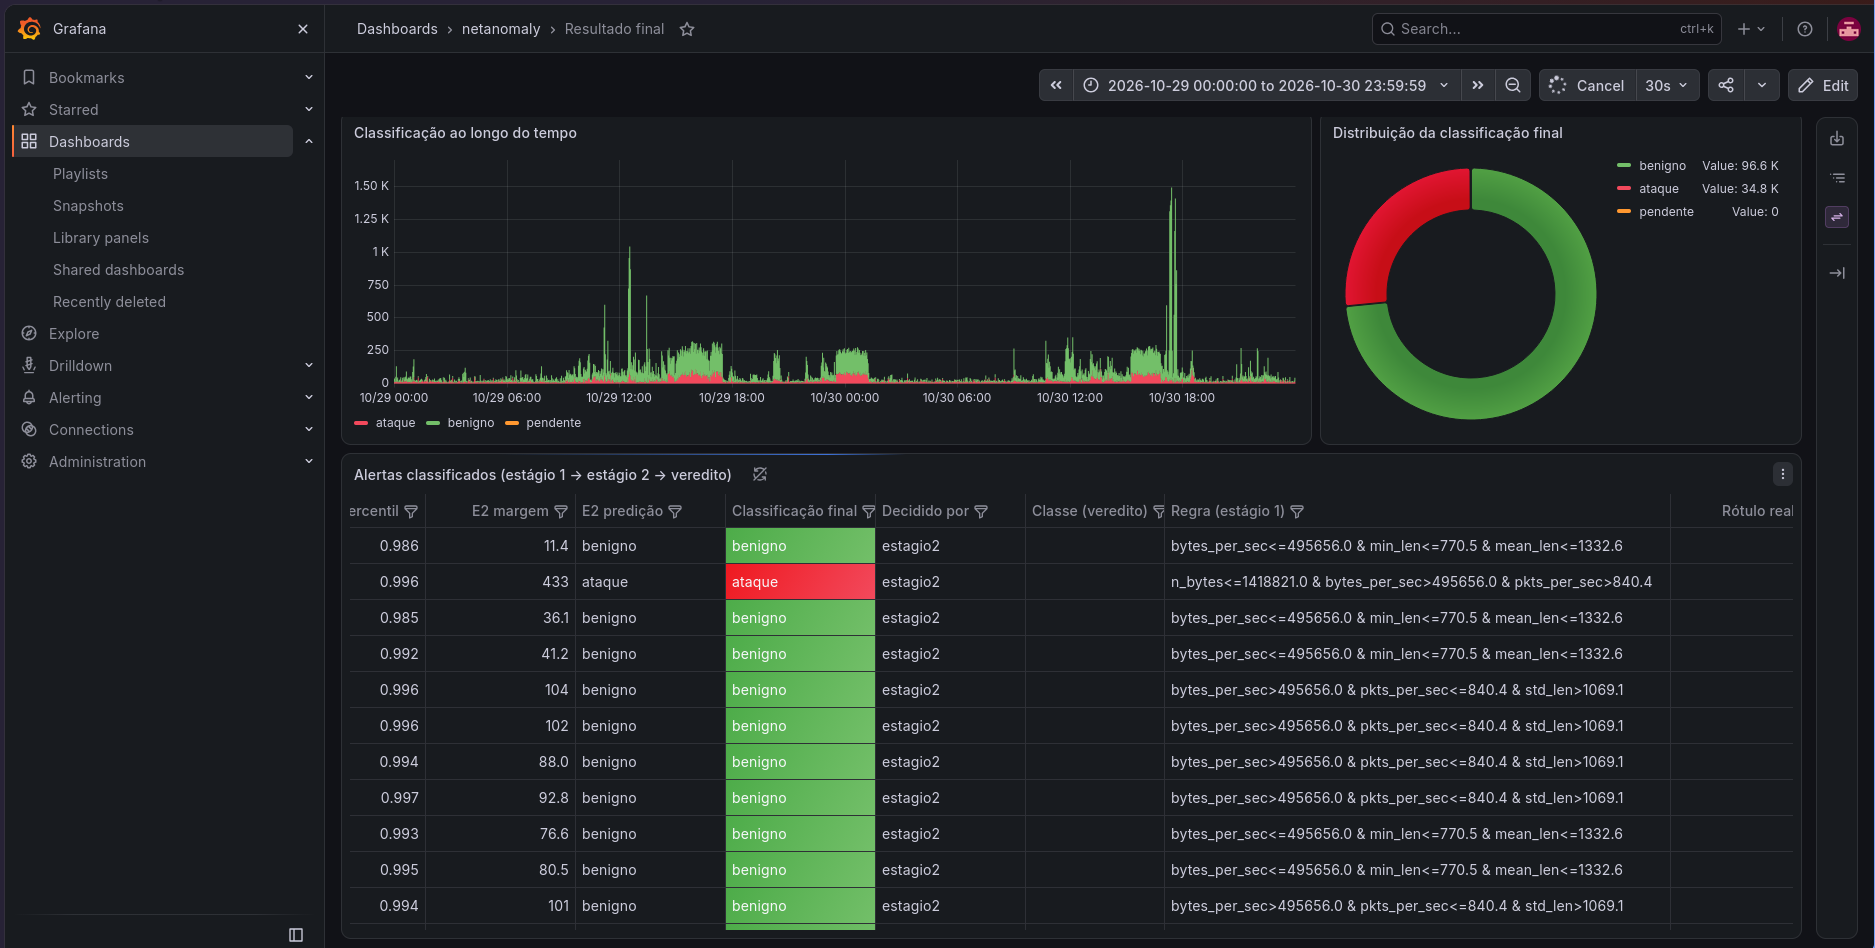
\includegraphics[width=\linewidth]{analista.png}
  \caption{}
  \label{fig:janela_analista}
\end{figure}


\textbf{Estágio 2 --- refinador supervisionado.} O Estágio 2 usa
\texttt{StandardScaler} e \texttt{LinearSVC} com $C=1$ e \texttt{class\_weight="balanced"}.
Os atributos de entrada são os 17 do fluxo.
O $SVM$ linear foi escolhido, em vez de uma clusterização pura, pois sua
\texttt{decision\_function} fornece a distância com sinal ao hiperplano, usada para
priorizar a revisão; a clusterização fica reservada como apoio à rotulagem em lote.

Uma instalação nova não tem nenhum veredito. O primeiro hiperplano é treinado sobre
o \textit{golden set} (capturas rotuladas como ataque ou benigno) e entra em produção
com a decisão registrada como \emph{adotado}. Os
vereditos do analista são somados ao treino à medida que chegam e valem como rótulo
da rede real.

O treinador aplica o SVM promovido aos alertas novos a cada 30~s, gravando a classe
predita, o valor de decisão e a margem. A fila de revisão é ordenada por margem
crescente: os casos mais próximos da fronteira aparecem primeiro, que é onde o
veredito mais move o hiperplano. Para o painel, uma projeção PCA em duas dimensões é
ajustada no treino e congelada no artefato (Figura \ref{fig:pca_pipeline}), de modo
que pontos de janelas diferentes sejam comparáveis.

\begin{figure}[H]
  \centering
  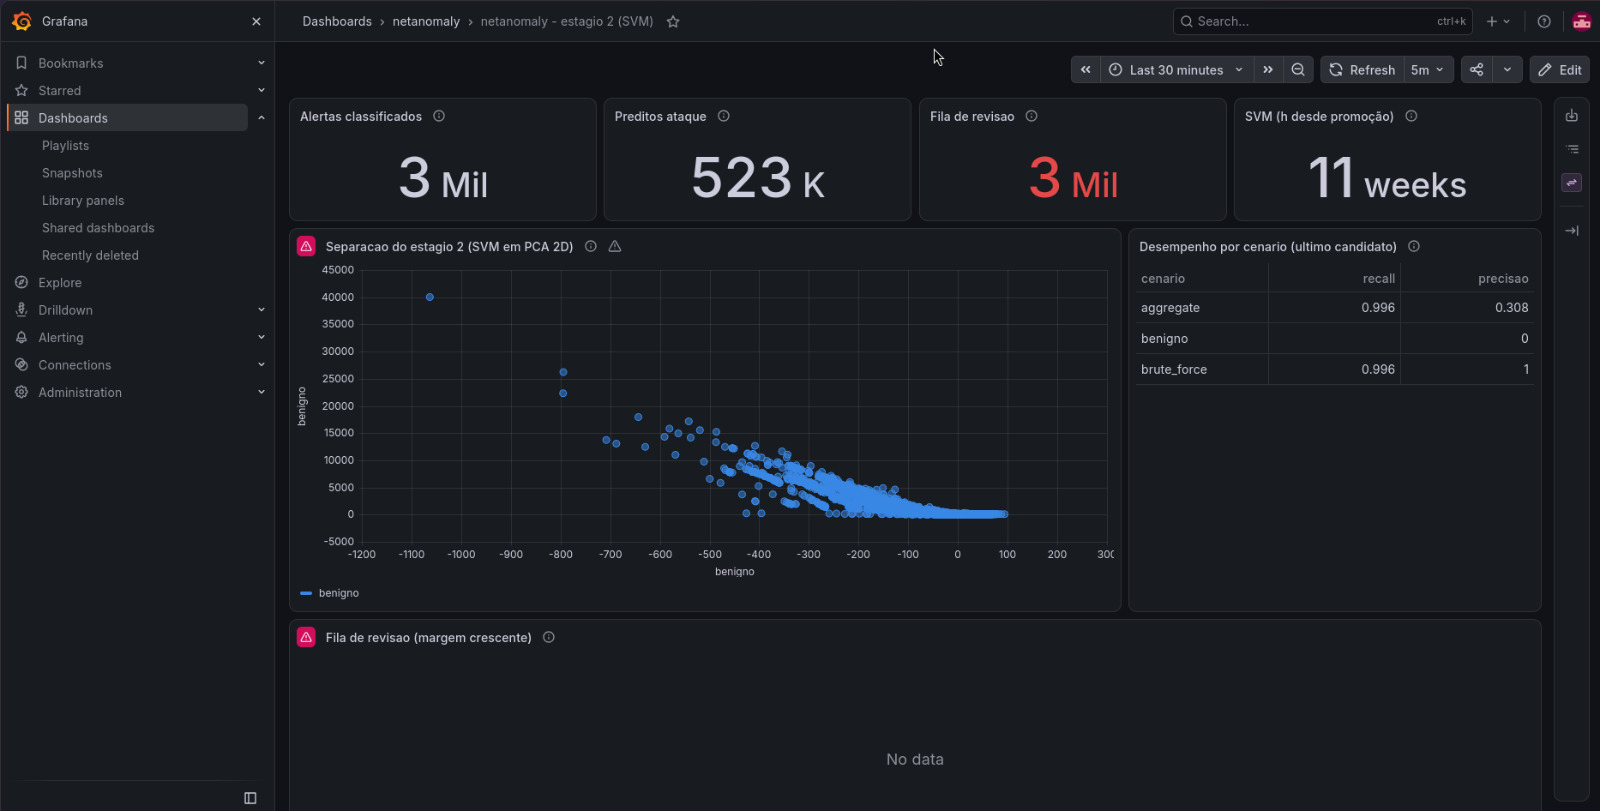
\includegraphics[width=\linewidth]{pca2d-dashboard.jpg}
  \caption{Projeção PCA 2D congelada no artefato do Estágio 2, usada no painel: golden set do CIC-IDS-2017 por classe.}
  \label{fig:pca_pipeline}
\end{figure}

\subsubsection{Governança de Dados, Resiliência a Envenenamento e Esteira de Validação}

\textbf{Ciclo de vida e \textit{pool} de treino.} A decisão central é que o detector
\textbf{não é retreinado na janela de tráfego mais recente}. O
\textit{Isolation Forest} aprende como normal a massa dos dados que recebe; se a janela
contém ataque, ele passa a ser normal e deixa de ser marcado. Isso é
explorável de forma gradual: um canal de comando e controle (C2) com batida de 6~h
é absorvido um pouco mais a cada retreino, sem que o atacante precise evadir nada
. O que o dado recente compra de fato é redução de falso
positivo (servidor novo, mudança de horário de \textit{backup}). Por isso o treino
ocorre sobre um \textit{pool} curado (Figura \ref{fig:ciclo}):

\begin{itemize}
  \item \textbf{Quarentena:} a janela só entra no \textit{pool} depois de 7 dias sem
  indicador de comprometimento ($IOC$) retroativo.
  \item \textbf{Recência:} cada janela recebe peso
  $w = 0{,}5^{\,(t_{\max}-t)/h}$, com meia-vida $h = 14$ dias, normalizado pela
  janela mais nova do \textit{pool}. Janelas com $w < 0{,}05$ são descartadas. A
  amostragem (limitada a 2 milhões de linhas) é proporcional ao tamanho da janela e
  serve só para limitar memória; a recência entra pelo \texttt{sample\_weight},
  para não ser duplicada.
  \item \textbf{Despejo e procedência:} cada modelo registra quais janelas o
  treinaram. Descoberto um comprometimento, as janelas do período são despejadas,
  a consulta \texttt{v\_models\_contaminados} lista os modelos que as absorveram e um
  novo candidato é treinado sem elas.
  \item \textbf{Homogeneidade:} janelas com contratos de atributos diferentes não
  são misturadas, pois geraria um modelo cujo vetor de entrada não existe.
\end{itemize}
\begin{figure}[H]
  \centering
  % Estados de uma janela de tráfego e os três relógios do ciclo de vida
\resizebox{\columnwidth}{!}{%
\begin{tikzpicture}[
  node distance=0.45cm and 0.55cm,
  every node/.style={font=\scriptsize},
  est/.style={rectangle, draw, rounded corners=6pt, fill=azulFEI!8,
              text width=1.6cm, align=center, minimum height=0.8cm, inner sep=2pt},
  mau/.style={est, fill=red!10},
  arrow/.style={-{Stealth[length=4pt]}},
  lbl/.style={font=\tiny, align=center}
]
  \node (jan)  [est] {Janela capturada (13 min)};
  \node (qua)  [est, right=of jan] {Quarentena};
  \node (ati)  [est, right=of qua] {\textit{Pool} ativo};
  \node (pes)  [est, right=of ati] {Peso $\to$ 0 (cauda)};
  \node (des)  [mau, below=0.9cm of ati] {Despejada};
  \node (mod)  [mau, right=of des] {Modelos contaminados};

  \draw[arrow] (jan) -- (qua);
  \draw[arrow] (qua) -- node[lbl, above,yshift=4pt]{7 dias sem\\IOC} (ati);
  \draw[arrow] (ati) -- node[lbl, above,yshift=8pt]{$w<0{,}05$} (pes);
  \draw[arrow] (qua.south) |- node[lbl, pos=0.3, left]{IOC\\retroativo} (des.west);
  \draw[arrow] (ati) -- node[lbl, right]{IOC} (des);
  \draw[arrow] (des) -- node[lbl, below,yshift=-9pt]{procedência} (mod);
\end{tikzpicture}%
}

  \caption{Estados de uma janela de tráfego no \textit{pool} de treino.}
  \label{fig:ciclo}
\end{figure}

\textbf{\textit{Benchmark} do \textit{golden set}.} O \textit{golden set} é um conjunto de
capturas rotuladas, organizado por cenário (Tabela \ref{tab:cenarios}), contra o
qual todo candidato é avaliado por captura, por cenário e no agregado. As capturas
podem ser registradas manualmente, a partir de testes de intrusão feitos pelo
próprio operador, ou derivadas do cronograma oficial de ataques do CIC-IDS-2017
. Cada cenário tem um piso absoluto de \textit{recall} por estágio. Os pisos são definidos por estágio porque o
\textit{Isolation Forest} é estruturalmente cego a ataques volumosos e homogêneos. 
O Estágio 1 é cobrado de varredura e falso positivo, e
os ataques densos são cobrados do Estágio 2.


\begin{table}[H]
\centering
\footnotesize
\setlength{\tabcolsep}{3pt}
\begin{tabularx}{\columnwidth}{l X c c}
\toprule
\textbf{Cenário} & \textbf{Descrição} & \textbf{E1} & \textbf{E2} \\
\midrule
recon        & Varredura de portas e \textit{hosts} (nmap) & 0,90$^*$ & 0,90 \\
brute\_force & Força bruta em SSH, FTP, HTTP & --- & 0,85 \\
exfil        & Exfiltração por canal incomum & --- & 0,80 \\
beacon\_1h   & C2 com batida horária & --- & 0,75 \\
beacon\_6h   & C2 com batida de 6~h & --- & 0,60 \\
lateral      & Movimento lateral (SMB, RDP) & --- & 0,80 \\
benigno      & Controle limpo: mede falso positivo & FPR & FPR \\
\bottomrule
\end{tabularx}
\caption{Cenários do \textit{golden set} e piso de \textit{recall} exigido por estágio. $^*$não obrigatório até haver captura real.}
\label{tab:cenarios}
\end{table}

Duas fontes de dados alimentam as avaliações. As capturas
reais do CIC-IDS-2017 medem detecção. Um gerador sintético
(\texttt{scripts/gerar\_sintetico.py}) produz \textit{pools} e capturas de varredura,
beacon e tráfego normal com distribuições controladas; os números obtidos com ele
medem o mecanismo (portão, quarentena, despejo). Os experimentos de envenenamento usam 5 sementes, com o gerador
re-semeado antes de cada \textit{pool}, porque seu estado compartilhado faria a
composição do \textit{pool} depender da ordem das chamadas.
%NOTE: não tenho certeza se devemos manter o paragrafo de envenenamento a cima

\textbf{Automação da avaliação de candidatos.} O ciclo é regido por três relógios
separados. A árvore \textit{surrogate} acompanha cada modelo. Uma vez por dia, o
serviço \texttt{treinador} processa a fila de pedidos de retreino do analista e treina
um candidato sobre o \textit{pool} vigente, avalia-o contra o \textit{golden set} e grava o
resultado. A promoção para produção é
semanal ou sob demanda e \textbf{sempre manual}. O portão, implementado como
consulta (\texttt{v\_gate\_verdict}), reprova o candidato se qualquer cenário
isolado:

\begin{enumerate}
  \item cair mais de 0,10 de \textit{recall} em relação ao modelo em produção;
  \item ficar abaixo do piso absoluto do cenário para aquele estágio; ou
  \item exceder 2\% de falso positivo no controle benigno.
\end{enumerate}

O terceiro critério impede que um candidato, que alerta em tudo, passe
com \textit{recall} 1,00 em todos os cenários. A avaliação é por cenário, e não
agregada, porque o envenenamento lento aparece como a queda de um cenário
específico, que a média esconde. A promoção é manual porque um portão que se
auto-aprova vale apenas o que vale a cobertura do \textit{golden set}: com poucos
cenários, daria aparência de verificação ao que não foi verificado. Ao promover, o modelo anterior e as árvores que o descreviam são
aposentados e o artefato é trocado por \texttt{rename()} atômico de um \textit{symlink},
que o detector recarrega sem reinício. O Estágio 2 segue o mesmo ciclo
(candidato, avaliação em partição retida de 30\%, promoção).

\section{Resultados}
Os resultados estão organizados nas duas fases do trabalho. No MVP1, os
classificadores são comparados na base NSL-KDD, e os números servem para escolher o
algoritmo e os atributos. No MVP2, a cascata de dois estágios é avaliada de duas
formas: com métricas medidas \textit{offline} sobre o \textit{golden set} rotulado
(CIC-IDS-2017) e com a operação do sistema em tráfego real no laboratório, onde não
existe rótulo e o resultado é apresentado por estudo de caso. Todas as métricas e
figuras desta seção são geradas pelo \textit{notebook}
\texttt{notebooks/graficos\_modelos.ipynb}, com \texttt{random\_state = 42}.

\subsection{MVP1}

\subsubsection{Análise de Dados e Pré-processamento}
A base NSL-KDD contém os ataques listados na Tabela \ref{tab:ataquesXcategoria}.
Alguns dos rótulos não descrevem ataques propriamente ditos, mas ferramentas ou ações
(\textit{loadmodule}, \textit{perl}, \textit{nmap}); no contexto desta análise, foram
tratados como ataque. Para facilitar a leitura, os ataques foram agrupados nas
categorias \textit{normal}, \textit{DoS}, \textit{probe}, \textit{r2l} e \textit{u2r}.

\begin{table}[H]
\centering
\footnotesize
\begin{tabular}{|c|c|c|}
	\hline
	\textbf{Categoria} & \textbf{Tipos de Ataque} & \textbf{Qtd. de registros}\\
	\hline
	normal & normal & 67.343 \\
	\hline
	DoS &
	\begin{tabular}[c]{@{}c@{}} neptune, smurf, teardrop, \\ pod, land \end{tabular}
	& 44.971 \\
	\hline
	probe &
	\begin{tabular}[c]{@{}c@{}} nmap, ipsweep, satan \end{tabular}
	& 8.725 \\
	\hline
	r2l &
	\begin{tabular}[c]{@{}c@{}} warezclient, warezmaster, \\ guess\_passwd, imap, ftp\_write, \\ multihop, phf, spy \end{tabular}
	& 995 \\
	\hline
	u2r &
	\begin{tabular}[c]{@{}c@{}} buffer\_overflow, rootkit, \\ loadmodule, perl \end{tabular}
	& 52 \\
	\hline
\end{tabular}
\caption{Tipos de ataque agrupados por categoria (\texttt{KDDTrain+}).}
\label{tab:ataquesXcategoria}
\end{table}

A matriz de correlação (Figura \ref{fig:matriz_corr}) mostra que os atributos de
contagem de conexões e de taxa de erro são os mais correlacionados entre si, o que
indica redundância e motiva a redução de dimensionalidade.

\begin{figure}[H]
\centering
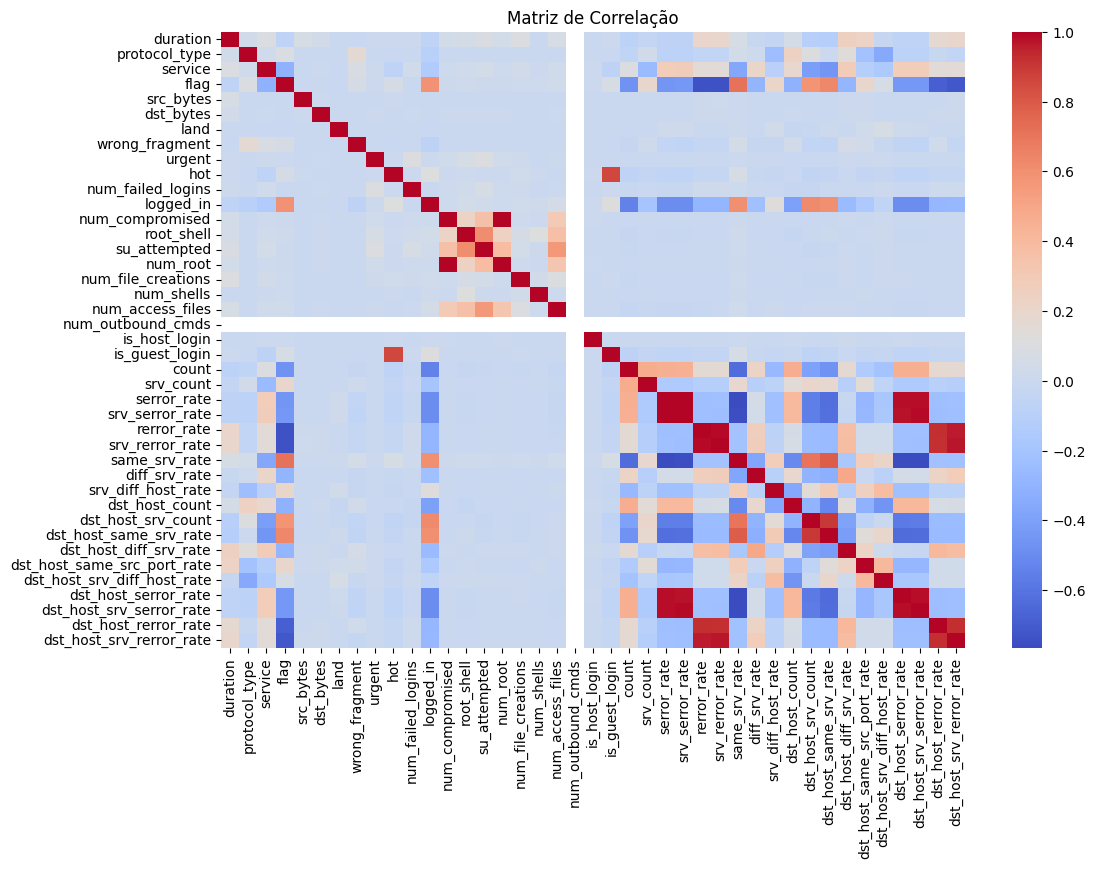
\includegraphics[width=8cm,height=8cm]{matriz_corr.png}
\caption{Matriz de correlação da base NSL-KDD.}
\label{fig:matriz_corr}
\end{figure}

Para validar essa leitura, a Figura \ref{fig:pca_componentes} projeta os registros
nas duas primeiras componentes do PCA, separados pelas categorias da Tabela
\ref{tab:ataquesXcategoria}, e a Figura \ref{fig:pca_ataqueXnormal} mostra a mesma
projeção apenas com as classes normal e ataque. A separação já é visível em duas
dimensões para \textit{DoS} e \textit{probe}; \textit{r2l} e \textit{u2r} ficam
sobrepostas ao tráfego normal, o que antecipa a dificuldade dos classificadores nessas
categorias.

\begin{figure}[H]
	\centering
	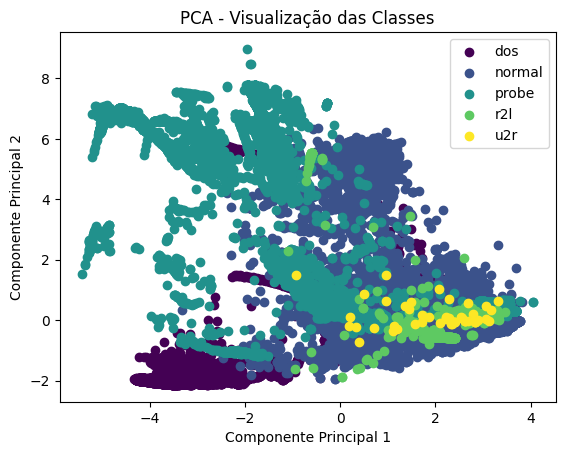
\includegraphics[width=8.69cm,height=7cm]{pca_classes.png}
	\caption{Duas primeiras componentes do PCA, separadas por categoria.}
	\label{fig:pca_componentes}
\end{figure}

\begin{figure}[H]
	\centering
	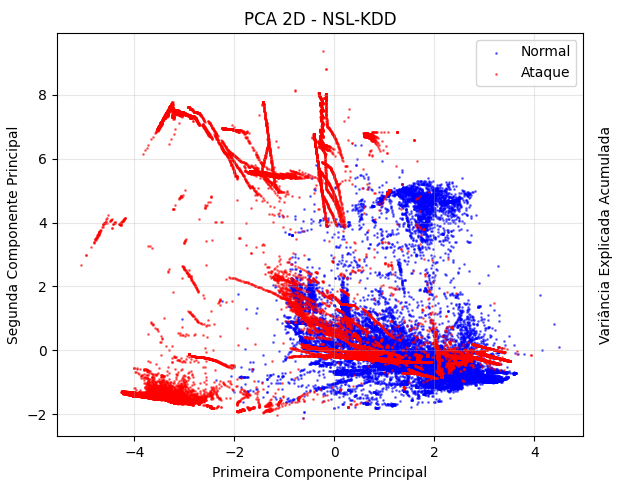
\includegraphics[width=8.69cm,height=7cm]{./PCA_2D.png}
	\caption{Duas primeiras componentes do PCA: ataque e tráfego normal.}
	\label{fig:pca_ataqueXnormal}
\end{figure}

\subsubsection{Comparação dos classificadores}
Os cinco classificadores ($Random Forest$ [RF], $Decision Tree$ [DT], KNN com
$k=5$, $Logistic Regression$ [LR] e SVM linear) foram treinados com os 41 atributos
padronizados e avaliados em dois conjuntos: a partição retida de 30\% do
\texttt{KDDTrain+} (Tabela \ref{tab:Tempos_treino}) e o \texttt{KDDTest+}, o conjunto
de teste oficial (Tabela \ref{tab:kddtest}).

\begin{table}[H]
	\centering
	\footnotesize
	\setlength{\tabcolsep}{2pt}
	\begin{tabular}{|l|c|c|c|c|c|c|}
		\hline
		\textbf{Modelo} & \textbf{Acc} & \textbf{Prec} & \textbf{Rec} & \textbf{F1} & \textbf{T. treino (s)} & \textbf{T. teste (s)} \\
		\hline
		RF  & 0,9990 & 0,9995 & 0,9984 & 0,9989 & 1,729   & 0,0369 \\
		DT  & 0,9981 & 0,9981 & 0,9977 & 0,9979 & 0,601   & \textbf{0,0038} \\
		KNN & 0,9958 & 0,9955 & 0,9956 & 0,9955 & 0,005   & 2,567 \\
		LR  & 0,9537 & 0,9597 & 0,9399 & 0,9497 & 2,696   & 0,0085 \\
		SVM & 0,9596 & 0,9662 & 0,9462 & 0,9561 & 154,420 & 7,663 \\
		\hline
	\end{tabular}
	\caption{Métricas na partição retida (30\% do \texttt{KDDTrain+}, 37.792 registros). Acc = acurácia, Prec = precisão, Rec = \textit{recall}.}
	\label{tab:Tempos_treino}
\end{table}

Na partição retida, todos os modelos baseados em árvore e o KNN ficam acima de
99,5\% de acurácia. Esse resultado é otimista porque treino e teste vêm do mesmo
arquivo: os mesmos tipos de ataque aparecem nos dois lados. O \texttt{KDDTest+} traz
17 tipos de ataque ausentes do treino e, por isso, mede a generalização. Nele, todos
os modelos perdem entre 16 e 23 pontos de acurácia, e a diferença entre eles aparece.

\begin{table}[H]
	\centering
	\footnotesize
	\setlength{\tabcolsep}{3pt}
	\begin{tabular}{|l|c|c|c|c|c|c|}
		\hline
		\textbf{Modelo} & \textbf{Acc} & \textbf{Prec} & \textbf{Rec} & \textbf{F1} & \textbf{FPR} & \textbf{MCC} \\
		\hline
		RF  & 0,7650 & 0,9668 & 0,6081 & 0,7466 & 0,0276 & 0,5996 \\
		DT  & \textbf{0,8348} & 0,9706 & \textbf{0,7320} & \textbf{0,8346} & 0,0293 & \textbf{0,7030} \\
		KNN & 0,7686 & 0,9704 & 0,6122 & 0,7508 & 0,0247 & 0,6064 \\
		LR  & 0,7519 & 0,9250 & 0,6140 & 0,7380 & 0,0658 & 0,5598 \\
		SVM & 0,7568 & 0,9647 & 0,5945 & 0,7356 & 0,0287 & 0,5871 \\
		\hline
	\end{tabular}
	\caption{Métricas no \texttt{KDDTest+} (22.544 registros, com ataques inéditos). FPR = taxa de falso positivo; MCC = coeficiente de correlação de Matthews.}
	\label{tab:kddtest}
\end{table}

A $Decision Tree$ é o modelo com melhor generalização: 0,8348 de acurácia e 0,732 de
\textit{recall} no \texttt{KDDTest+}, 12 pontos acima do segundo colocado em
\textit{recall}, com o menor tempo de teste entre os cinco (3,8~ms para 37.792
registros). A Figura \ref{fig:recall_categoria} mostra de onde vem a vantagem: nas
categorias minoritárias, a DT detecta 39\% dos ataques \textit{r2l} contra no máximo
12\% dos demais modelos, e 40\% dos \textit{u2r}. Em todos os modelos, \textit{r2l} e
\textit{u2r} continuam sendo as categorias mais difíceis, como já antecipava a
sobreposição observada no PCA.

\begin{figure}[H]
	\centering
	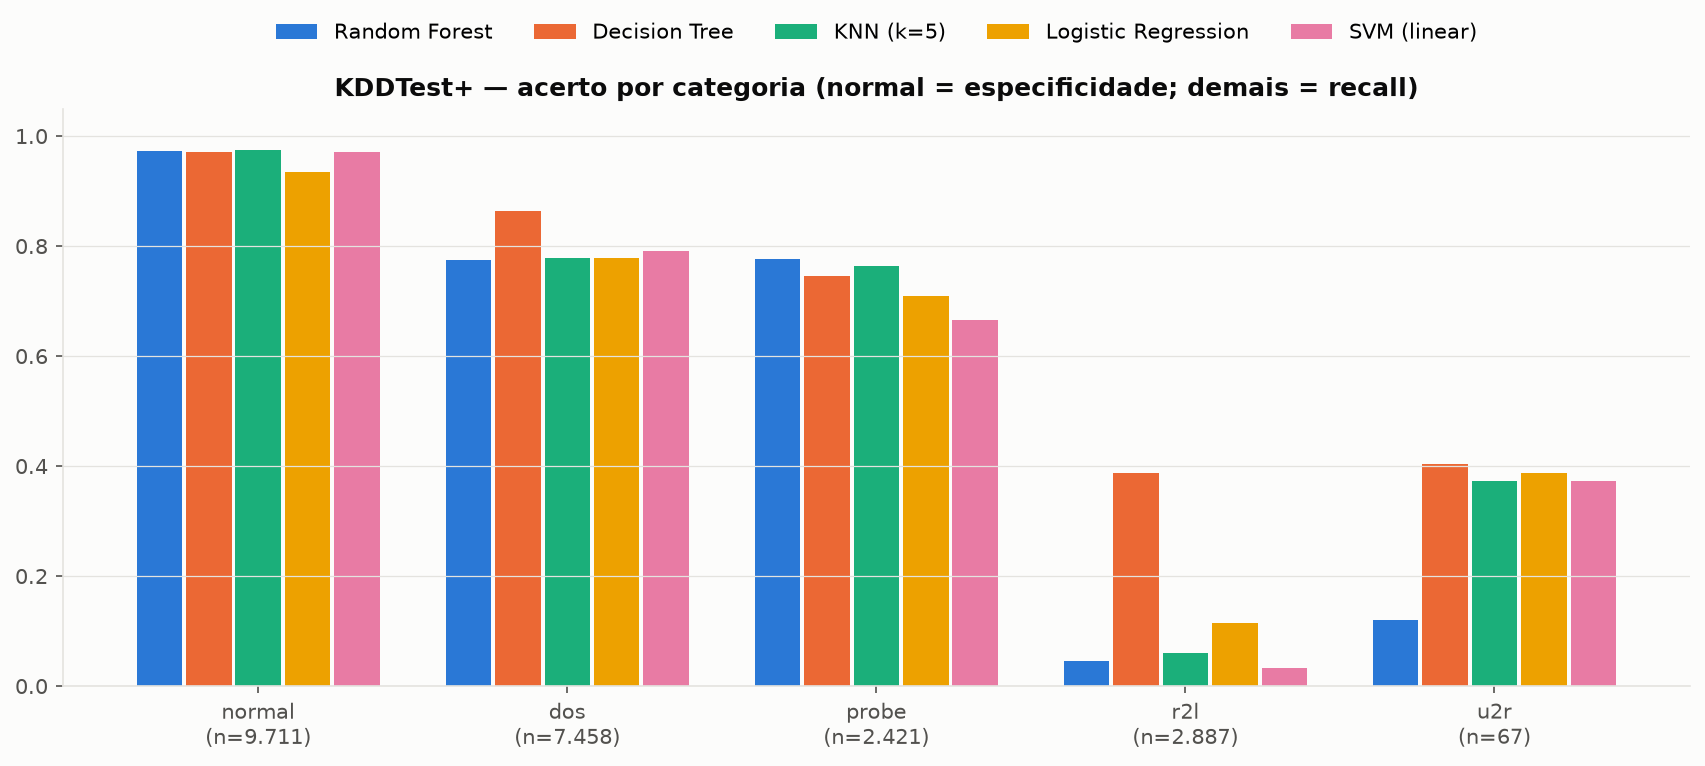
\includegraphics[width=\linewidth]{../../notebooks/figuras/A7_recall_por_categoria.png}
	\caption{Taxa de acerto por categoria no \texttt{KDDTest+} (normal = especificidade; demais categorias = \textit{recall}).}
	\label{fig:recall_categoria}
\end{figure}

A Figura \ref{fig:fronteiras} ilustra como cada família de modelo recorta o espaço.
Para que a fronteira possa ser desenhada, cada modelo foi retreinado apenas com PC1 e
PC2; a figura é ilustrativa e não corresponde aos modelos avaliados nas tabelas. A
árvore produz recortes ortogonais aos eixos, enquanto LR e SVM linear ficam limitados
a uma única reta.

\begin{figure}[H]
	\centering
	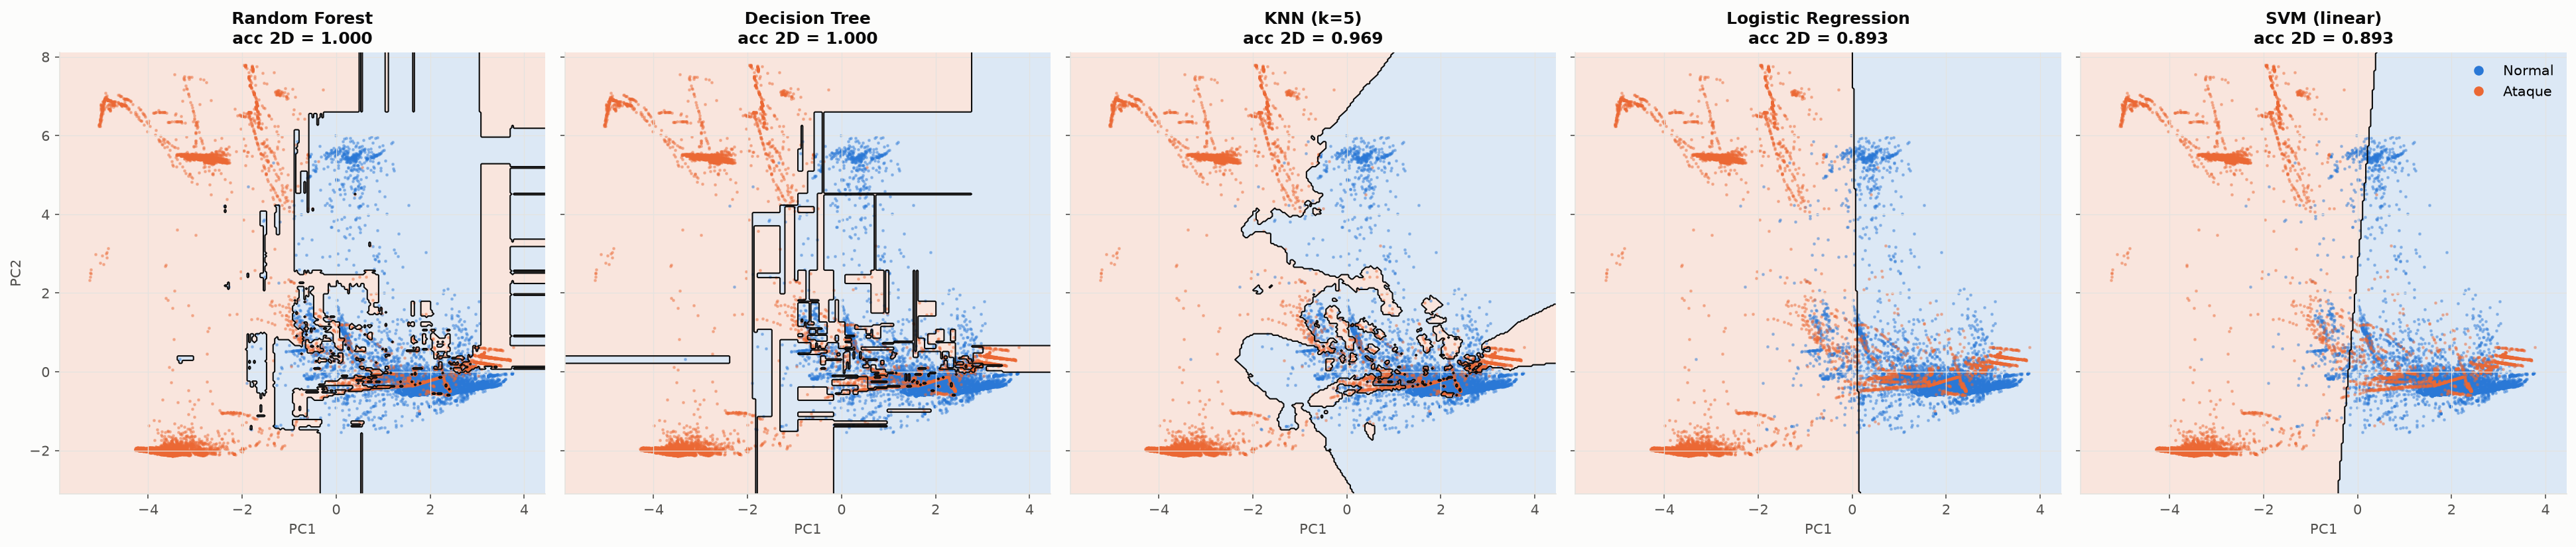
\includegraphics[width=\linewidth]{../../notebooks/figuras/A6_fronteiras_pca.png}
	\caption{Fronteiras de decisão de cada algoritmo no plano PC1 $\times$ PC2.}
	\label{fig:fronteiras}
\end{figure}

Como o objetivo do sistema é operar em tempo real, o critério de escolha combinou
generalização e custo de inferência. A $Decision Tree$ ficou em primeiro lugar nos
dois critérios e foi o algoritmo selecionado.

\subsubsection{Redução de Dimensionalidade e Seleção de Atributos}
Para preservar mais de 95\% da variância, o PCA precisa de 23 das 41 componentes
(Figura \ref{fig:pca_variancia}). A redução, porém, não favoreceu os classificadores:
no \texttt{KDDTest+}, o F1 da $Decision Tree$ caiu de 0,8346 com os 41 atributos para
0,7714 com as componentes do PCA, e o do $Random Forest$ caiu de 0,7466 para 0,7387.
Só a regressão logística teve ganho marginal (de 0,7380 para 0,7435). A projeção
mistura atributos com escalas e significados diferentes, e a árvore perde os cortes
diretos que fazia sobre atributos individuais.

\begin{figure}[H]
\centering
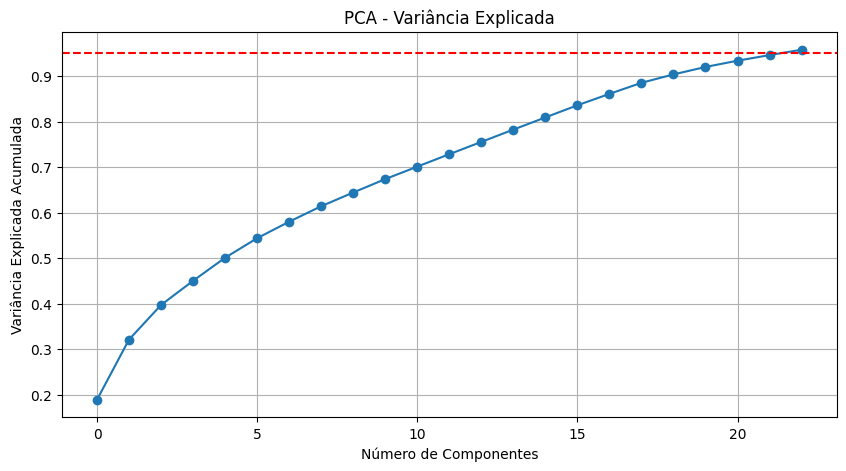
\includegraphics[width=8.5cm,height=5.5cm]{pcaXvariancia.png}
\caption{Variância explicada acumulada do PCA.}
\label{fig:pca_variancia}
\end{figure}

A seleção de atributos funcionou melhor que a projeção. As Figuras
\ref{fig:Importancia_features} e \ref{fig:DecisionTree_features} mostram a importância
de cada atributo e a acurácia da $Decision Tree$ treinada com os $k$ atributos mais
importantes: a curva se estabiliza acima de 95\% e atinge o máximo com 18 atributos.

\begin{figure}[H]
	\centering
	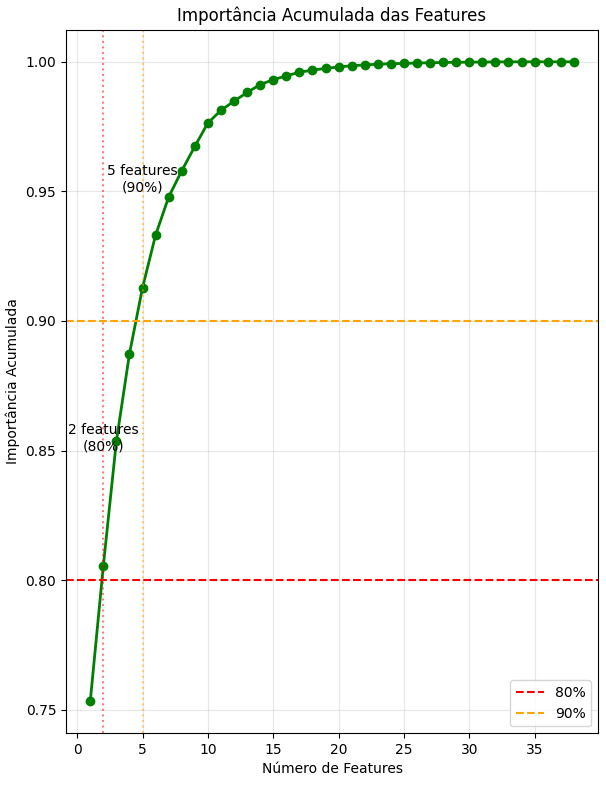
\includegraphics[width=8.69cm,height=11cm]{./Importancia_features.png}
	\caption{Importância de cada atributo.}
	\label{fig:Importancia_features}
\end{figure}

\begin{figure}[H]
	\centering
	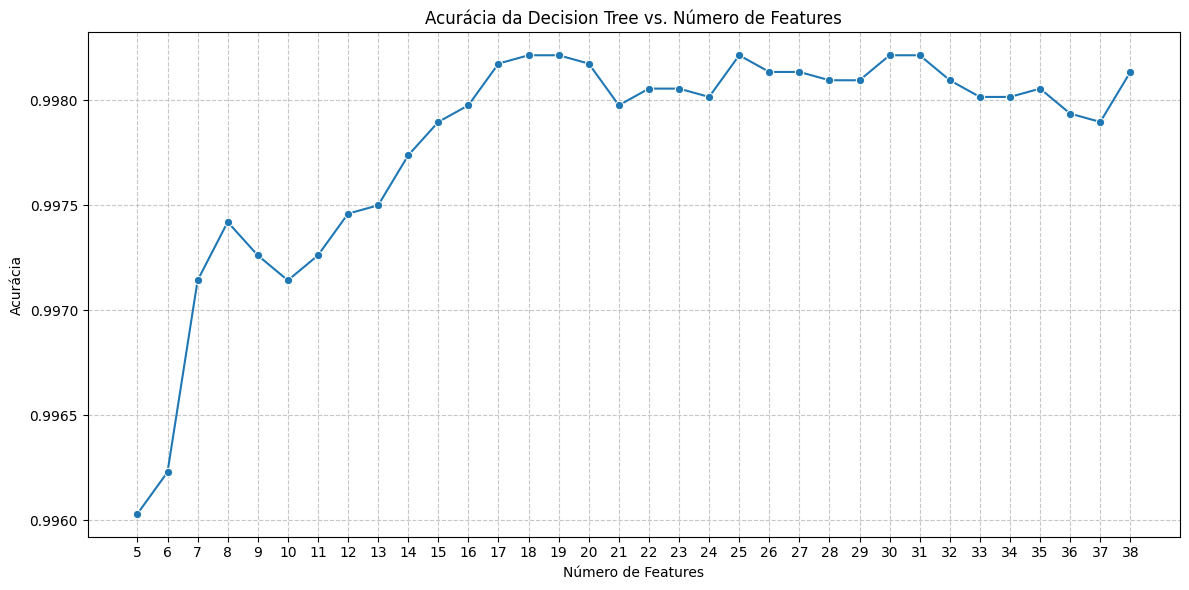
\includegraphics[width=9cm,height=6cm]{./decisiontree_features.png}
	\caption{Acurácia da $Decision Tree$ em função do número de atributos.}
	\label{fig:DecisionTree_features}
\end{figure}

Os 18 atributos selecionados são:
\begin{enumerate}
	\item \textbf{src\_bytes}: número de bytes enviados da origem para o destino.
	\item \textbf{dst\_host\_srv\_count}: quantidade de conexões para o mesmo serviço do destino (entre as últimas 100).
	\item \textbf{count}: número de conexões para o mesmo \textit{host} de destino nos últimos 2 segundos.
	\item \textbf{dst\_bytes}: número de bytes enviados do destino para a origem.
	\item \textbf{dst\_host\_srv\_rerror\_rate}: percentual de conexões recusadas entre as contadas em \textbf{dst\_host\_srv\_count}.
	\item \textbf{hot}: número de indicadores de acesso a diretórios do sistema ou de criação e execução de programas.
	\item \textbf{dst\_host\_same\_src\_port\_rate}: percentual de conexões que usam a mesma porta de origem da conexão atual.
	\item \textbf{logged\_in}: indicador binário de autenticação bem-sucedida.
	\item \textbf{srv\_count}: número de conexões para a mesma porta da conexão atual nos últimos 2 segundos.
	\item \textbf{dst\_host\_same\_srv\_rate}: percentual de conexões ao mesmo \textit{host} de destino que usam a mesma porta.
	\item \textbf{duration}: duração da conexão em segundos.
	\item \textbf{dst\_host\_rerror\_rate}: percentual de conexões recusadas.
	\item \textbf{dst\_host\_diff\_srv\_rate}: percentual de conexões para portas diferentes do mesmo destino.
	\item \textbf{dst\_host\_count}: número de conexões direcionadas ao mesmo IP de destino.
	\item \textbf{dst\_host\_serror\_rate}: percentual de conexões com erro do tipo $SYN$.
	\item \textbf{wrong\_fragment}: número de fragmentos corrompidos na conexão.
	\item \textbf{dst\_host\_srv\_diff\_host\_rate}: percentual de conexões para a mesma porta vindas de origens diferentes.
	\item \textbf{diff\_srv\_rate}: percentual de conexões para portas diferentes.
\end{enumerate}

Do MVP1, duas conclusões passaram ao MVP2: a ordem de grandeza do vetor de atributos
(17 atributos por fluxo) e a evidência de que volume, contagem e taxa de erro de
conexão são os sinais mais discriminantes.

\subsection{MVP2}
O MVP2 foi avaliado em duas frentes. A primeira é a avaliação \textit{offline} sobre
o \textit{golden set}: 14.615 fluxos do CIC-IDS-2017 rotulados pelo cronograma oficial
da base (875 de ataque e 13.740 de controle benigno do mesmo período). A segunda é a
operação do sistema em tempo real no laboratório, sobre o tráfego da rede
\texttt{192.168.60.0/24}.

\subsubsection{Estágio 1 --- \textit{Isolation Forest}}
O \textit{Isolation Forest} promovido ($c = 0{,}01$) marcou 0,87\% do \textit{pool}
de treino como alerta, coerente com o \textit{contamination} configurado. No
\textit{golden set}, porém, o \textit{recall} foi \textbf{zero}: nenhum dos 875 fluxos
de ataque ultrapassou o limiar, e 131 fluxos benignos foram marcados (FPR de 0,95\%),
como mostra a Figura \ref{fig:if_golden}. O ROC-AUC de 0,718 indica que o escore
ordena os ataques acima da maior parte do tráfego benigno, mas não acima do benigno
atípico, que é justamente o que o limiar seleciona.

\begin{strip}
\begin{figure}[H]
	\centering
	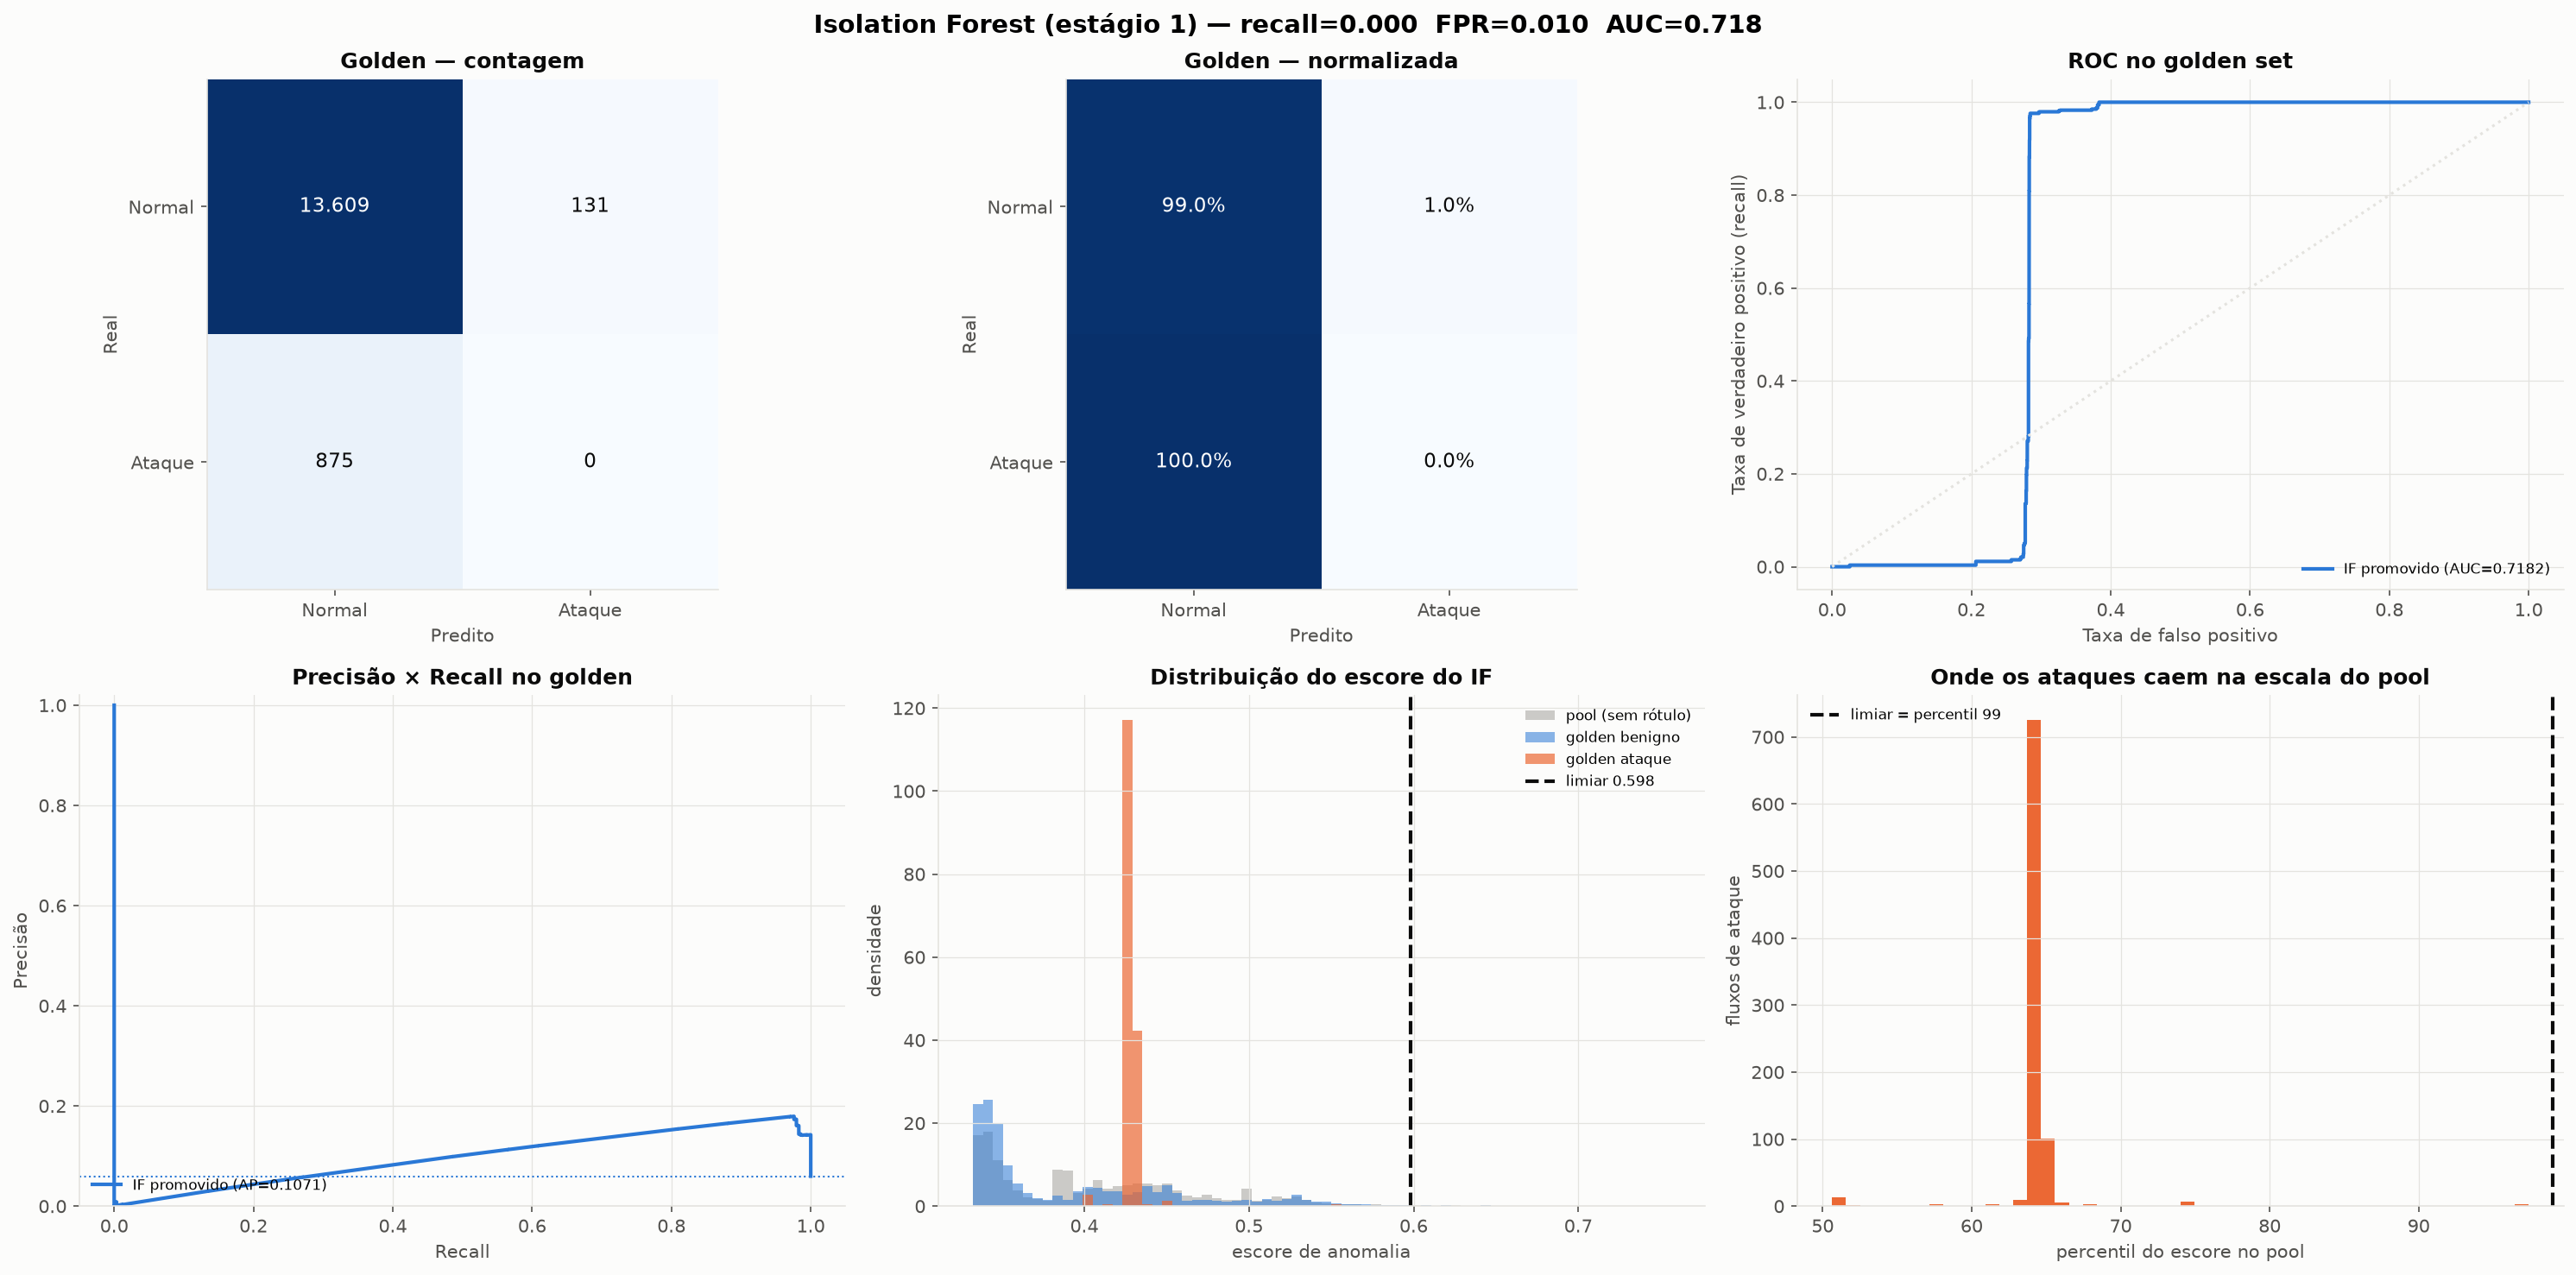
\includegraphics[width=\textwidth]{../../notebooks/figuras/B1_isolation_forest.png}
	\caption{Estágio 1 no \textit{golden set}: matriz de confusão, curvas ROC e PR, distribuição do escore e posição dos ataques na escala de percentil do \textit{pool}.}
	\label{fig:if_golden}
\end{figure}
\end{strip}

A causa é estrutural. O painel inferior direito da Figura
\ref{fig:if_golden} mostra que os ataques do \textit{golden set} se acumulam em um
pico estreito por volta do percentil 64 do \textit{pool}: são milhares de fluxos
quase idênticos, que formam um aglomerado denso. O \textit{Isolation Forest} isola
pontos \textbf{raros}, de modo que um ataque volumoso e homogêneo parece normal ao
detector, e parece mais normal quanto mais se repete. O histórico de candidatos
confirma isso: todos os 20 candidatos treinados com $c = 0{,}01$ ao longo do
projeto tiveram \textit{recall} de 0,000, e subir o \textit{contamination} para
0,03 elevou o \textit{recall} para apenas 0,003, com FPR entre 3,7\% e 5,5\%. O que justifica a existência de um segundo
estágio supervisionado.

A árvore \textit{surrogate} (Figura \ref{fig:arvore}) reproduz as decisões do
\textit{Isolation Forest} com 99,73\% de concordância no \textit{pool} (partição de
30\%, 60.000 fluxos). Ela recupera 75,2\% dos alertas do $IF$ e gera apenas 9 alertas
que o $IF$ não geraria (Figura \ref{fig:fidelidade}). As regras exibidas ao analista
explicam, portanto, a maior parte das decisões do detector, sobretudo por meio de
\texttt{n\_bytes}, \texttt{bytes\_per\_sec} e \texttt{syn\_no\_ack} (Figura \ref{fig:janela_analista})

\begin{figure}[H]
	\centering
	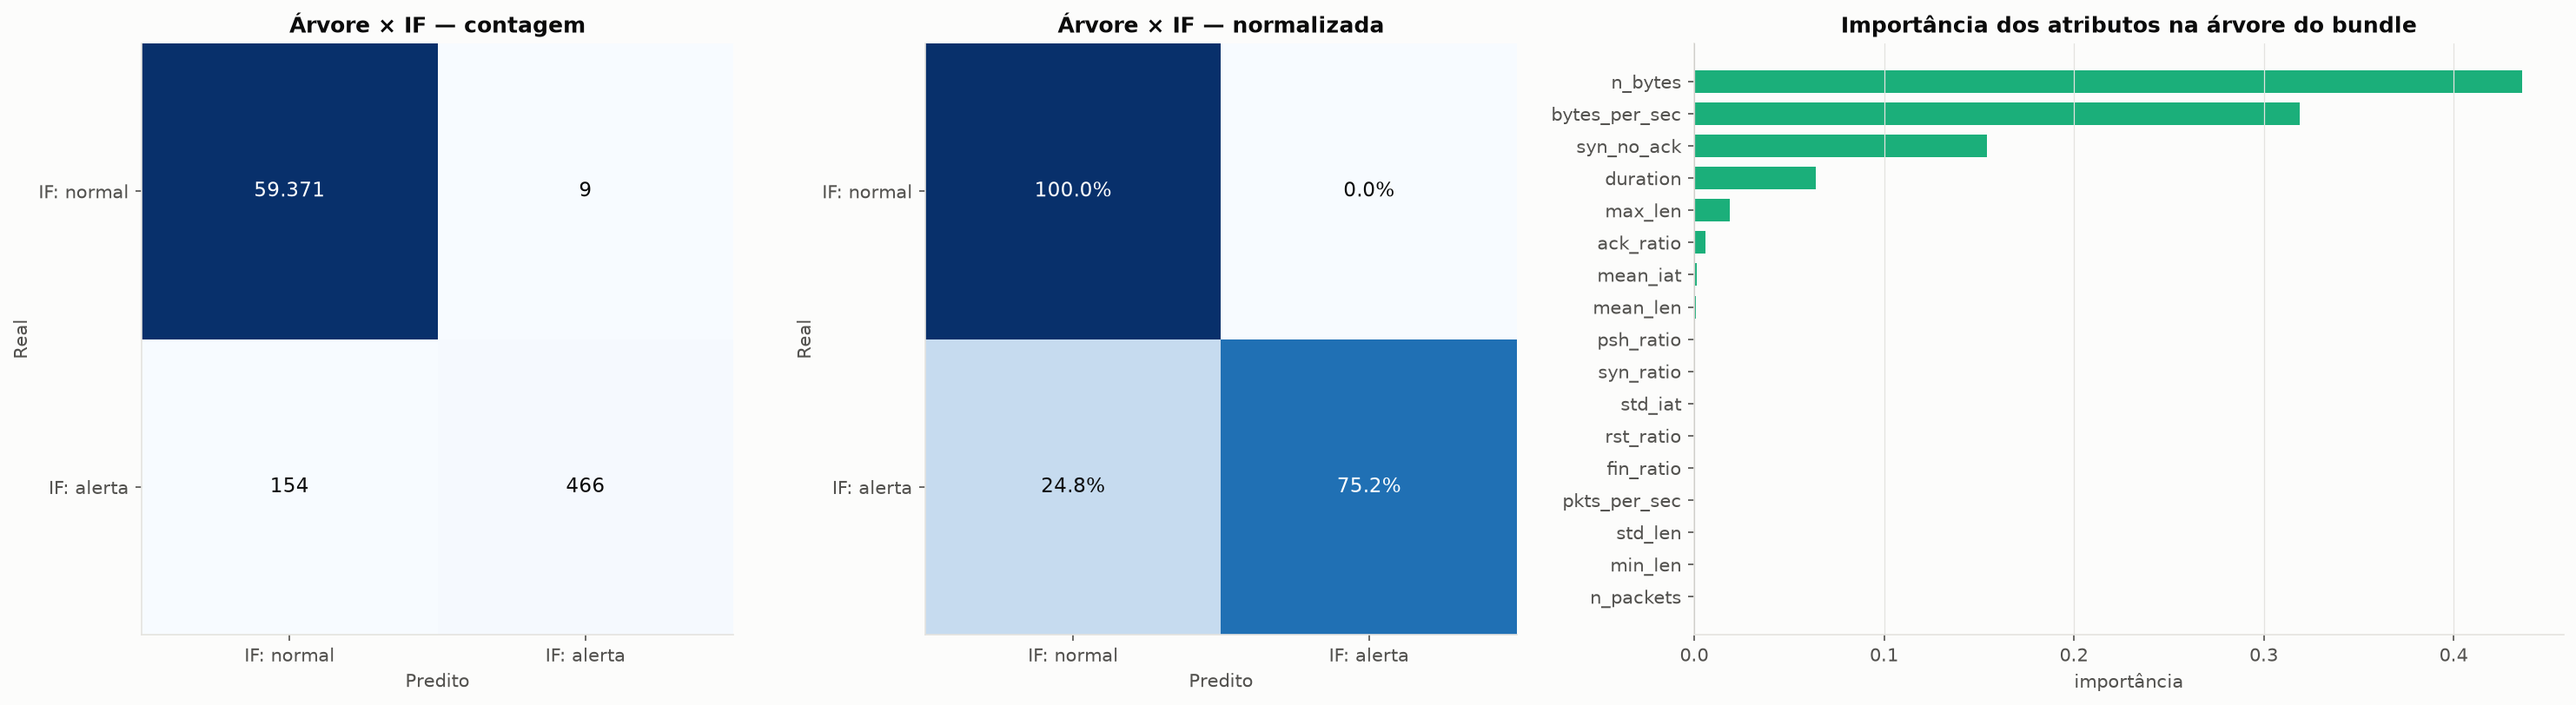
\includegraphics[width=\linewidth]{../../notebooks/figuras/B2_arvore_fidelidade.png}
	\caption{Fidelidade da árvore \textit{surrogate} ao \textit{Isolation Forest} e importância dos atributos.}
	\label{fig:fidelidade}
\end{figure}

\subsubsection{Estágio 2 --- SVM linear}
O estágio 2 (\texttt{StandardScaler} + \texttt{LinearSVC} com
\texttt{class\_weight="balanced"}) foi avaliado em uma partição estratificada de
30\% do \textit{golden set}, com o modelo treinado nos 70\% restantes. Os resultados
estão na Tabela \ref{tab:estagios} e na Figura \ref{fig:svm_golden}.

\begin{table}[H]
	\centering
	\footnotesize
	\setlength{\tabcolsep}{2.5pt}
	\begin{tabular}{|l|c|c|c|c|c|c|}
		\hline
		\textbf{Modelo} & \textbf{Prec} & \textbf{Rec} & \textbf{F1} & \textbf{FPR} & \textbf{AUC} & \textbf{MCC} \\
		\hline
		IF (estágio 1)        & 0,000 & 0,000 & 0,000 & 0,0097 & 0,7147 & $-$0,024 \\
		LinearSVC (estágio 2) & 0,910 & \textbf{1,000} & 0,953 & 0,0063 & 0,9996 & 0,951 \\
		\hline
		\multicolumn{7}{|l|}{\textit{Matriz do estágio 2: VP = 263, FP = 26, FN = 0, VN = 4.096}} \\
		\hline
	\end{tabular}
	\caption{Estágios 1 e 2 na mesma partição de teste (30\% do \textit{golden set}, 4.385 fluxos).}
	\label{tab:estagios}
\end{table}

Com os mesmos 17 atributos e os mesmos fluxos, o classificador supervisionado detecta
todos os 263 ataques da partição de teste, com 26 falsos positivos (0,63\%). O ROC-AUC
passa de 0,71 para 0,9996, e a precisão média (AP), de 0,107 para 0,989. A diferença
não está nos atributos, e sim no método: com o rótulo, o $SVM$ aprende a fronteira do
aglomerado denso que o \textit{Isolation Forest} trata como normal. O custo é baixo:
o treino levou 24~ms, e a predição dos 4.385 fluxos, menos de 1~ms.

\begin{strip}
\begin{figure}[H]
	\centering
	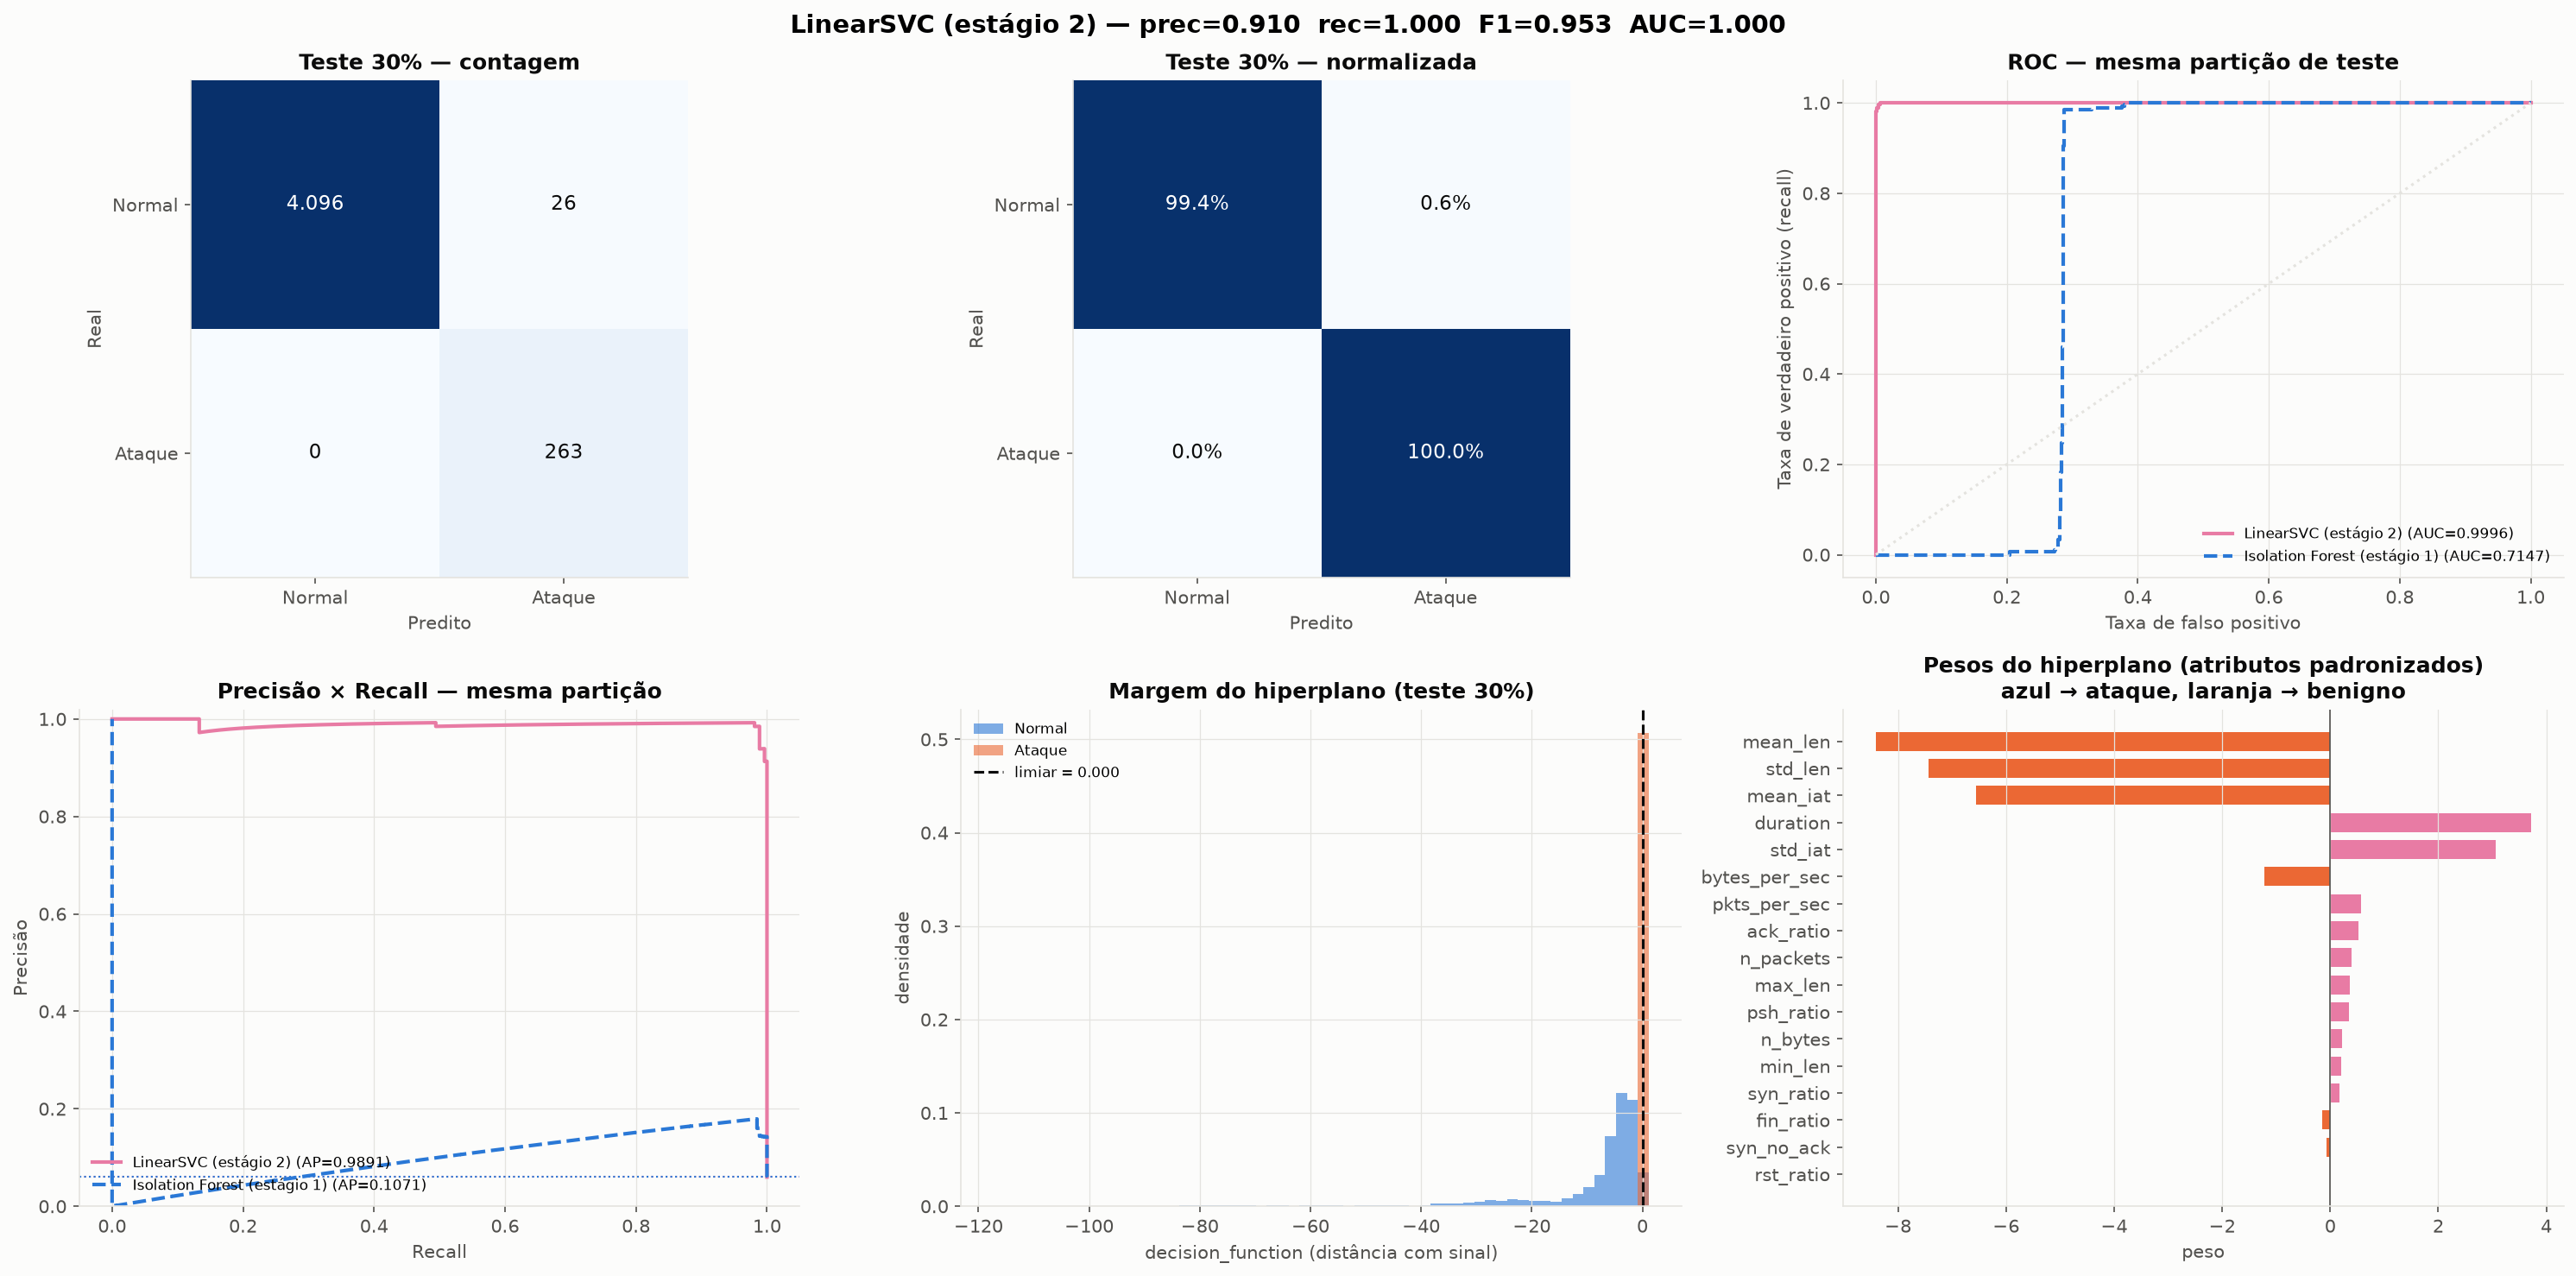
\includegraphics[width=\textwidth]{../../notebooks/figuras/B3_linearsvc.png}
	\caption{Estágio 2 na partição de teste: matriz de confusão, ROC e PR comparadas às do estágio 1, distribuição da margem e pesos do hiperplano.}
	\label{fig:svm_golden}
\end{figure}
\end{strip}
%FIXME: a cor do gráfico mencionado inferior direito está errada

Os pesos do hiperplano (painel inferior direito da Figura \ref{fig:svm_golden}) têm
leitura direta. Tamanho médio e desvio do tamanho dos pacotes (\texttt{mean\_len},
\texttt{std\_len}) e intervalo médio entre pacotes (\texttt{mean\_iat}) empurram o
fluxo para o lado benigno, enquanto duração (\texttt{duration}) e irregularidade
temporal (\texttt{std\_iat}) o empurram para o lado de ataque. O resultado descreve
uma sessão longa de pacotes pequenos e repetitivos, que é o perfil de um ataque
automatizado.

\textbf{Modelo em produção.} O SVM promovido no sensor (\texttt{192.168.60.33}) é
treinado sobre o \textit{golden set} somado aos vereditos do analista. Sobre os
14.100 fluxos rotulados disponíveis, ele classifica de forma errada 515 (3,7\%). As
métricas são \textit{in-sample}, pois esses dados entraram no treino, e servem apenas
como diagnóstico. As Figuras \ref{fig:SVM_hiperplano} e \ref{fig:SVM_hiperplano3D}
desenham o hiperplano em uma base alinhada a ele: o eixo horizontal é a distância com
sinal de cada fluxo ao hiperplano, e os demais eixos são componentes principais do
resíduo ortogonal. Os erros (marcados com X) concentram-se do lado de ataque, junto
ao hiperplano, e são fluxos benignos parecidos com o aglomerado de ataque, ou seja,
falsos positivos. Em um IDS, esse é o tipo de erro preferível ao falso negativo.

\begin{strip}
\begin{figure}[H]
\centering
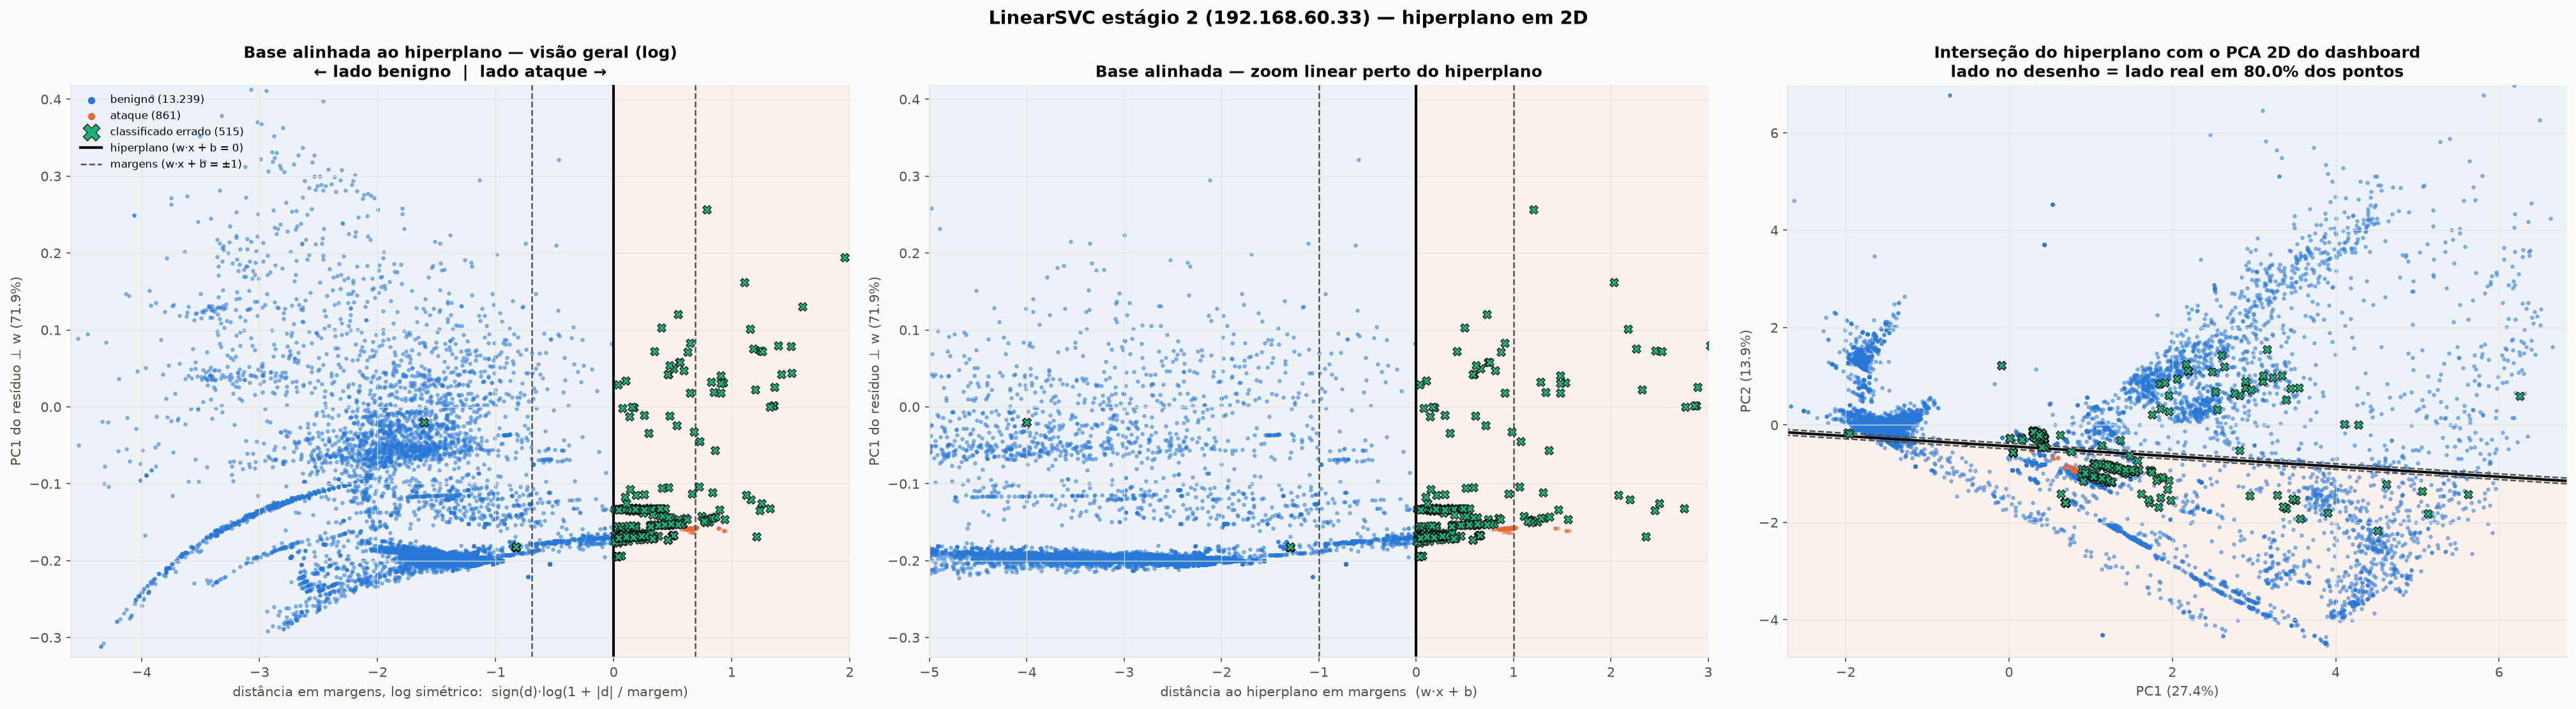
\includegraphics[width=\textwidth]{../../notebooks/figuras/B5_svm_hiperplano_2d_192_168_60_33.png}
\caption{Hiperplano do SVM em produção: base alinhada (visão geral em escala logarítmica e \textit{zoom} linear) e interseção com o PCA 2D do painel.}
\label{fig:SVM_hiperplano}
\end{figure}
\end{strip}

\begin{figure}[H]
\centering
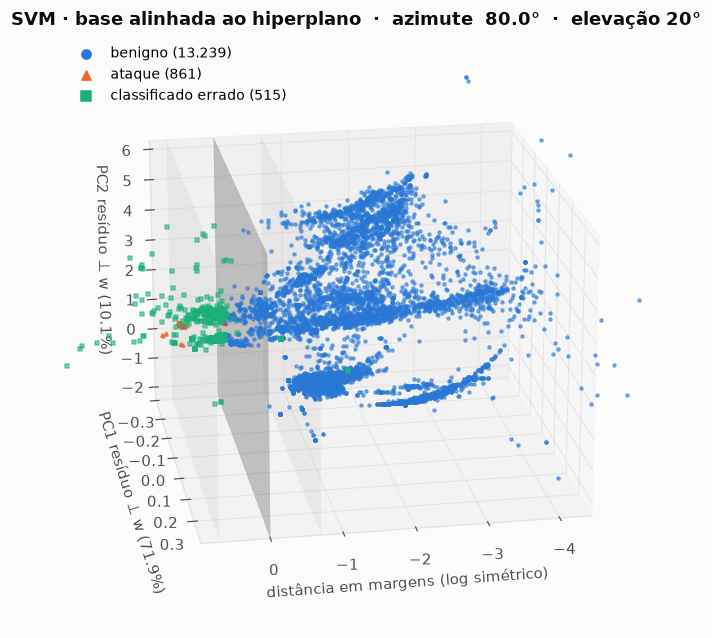
\includegraphics[width=\linewidth]{../../notebooks/figuras/svm360_alinhado_192_168_60_33/frame_032_az080.0.png}
\caption{Hiperplano do SVM em produção, em 3D (base alinhada).}
\label{fig:SVM_hiperplano3D}
\end{figure}

A projeção no PCA 2D usada no painel do Grafana (Figura \ref{fig:SVM_hiperplano},
painel direito) é aproximada: o lado do hiperplano em que o ponto aparece no desenho
coincide com o lado real em 80\% dos fluxos. Por isso, a decisão exibida ao analista
vem sempre da margem calculada nas 17 dimensões, e não da posição do ponto no
gráfico.

\textbf{Limite da cascata.} As métricas da Tabela \ref{tab:estagios} avaliam cada
estágio isoladamente. Em operação, o estágio 2 classifica apenas os fluxos gravados
como alerta pelo estágio 1, isto é, os que estão acima do piso de gravação (percentil
95). Os ataques do \textit{golden set}, concentrados em torno do percentil 64, não
chegariam ao estágio 2, e a cascata não os detectaria. O \textit{recall} de 1,000 do
$SVM$ indica que o classificador separa essa forma de ataque quando a recebe. Fechar essa lacuna exige atributos que
enxerguem a repetição, como a visão por \textit{host} da Tabela
\ref{tab:atributos}.

\subsubsection{Aplicação em tráfego real}
No tráfego de produção não existe rótulo: o painel \textit{Acerto vs. rótulo real}
indica \textit{sem rótulo} nos dois casos a seguir. A avaliação é feita, então, por
eventos cuja natureza é conhecida por construção: um evento benigno e incomum, e um
ataque executado de forma deliberada no laboratório. Os dois casos aparecem no painel
\textit{Resultado final}, que consolida, para cada alerta, a decisão do estágio 1, a
do estágio 2 e o veredito do analista, nessa ordem de precedência.

\textbf{Caso 1 --- anomalia benigna: reinício do modem.} Entre 00h00 e 12h50 de
18/09/2026, o estágio 1 gerou 373 alertas, todos classificados pelo estágio 2: 341
como benignos e 32 como ataque (Figura \ref{fig:anomalia_benigna}). O pico às 10h31,
com 46 alertas em uma única janela, coincide com o reinício do modem.

No laboratório, o modem e o roteador são equipamentos separados. O modem tem uma
rede exclusiva, e o roteador interliga essa rede à rede local
(\texttt{192.168.60.0/24}), onde está o sensor. Por isso, o reinício do modem
derrubou apenas o acesso à internet: a rede interna continuou funcionando
normalmente, sem perda de endereço nem de conectividade entre os \textit{hosts}
locais. O sensor, que observa a rede local, viu apenas o efeito da queda do link
externo: conexões com destinos na internet interrompidas, tentativas de reconexão
sem resposta durante a indisponibilidade e a retomada das sessões quando o modem
voltou. Esse padrão é atípico para a rede, e por isso o alerta do estágio 1 está
correto do ponto de vista estatístico. O estágio 2, porém, classificou os 46 fluxos
do pico como benignos, porque a forma desses fluxos não se parece com a dos ataques
que ele aprendeu.

O caso confirma a divisão de papéis prevista na arquitetura. Um detector não
supervisionado não sabe distinguir uma falha de infraestrutura de um ataque: os dois
são desvios em relação ao tráfego habitual. A falha de um enlace externo, que não
compromete a rede interna e não exige resposta de segurança, chegaria ao analista
como incidente se o sistema tivesse um único estágio. Com a cascata, ela é
registrada, mas não é classificada como ataque.

\begin{strip}
\begin{figure}[H]
	\centering
	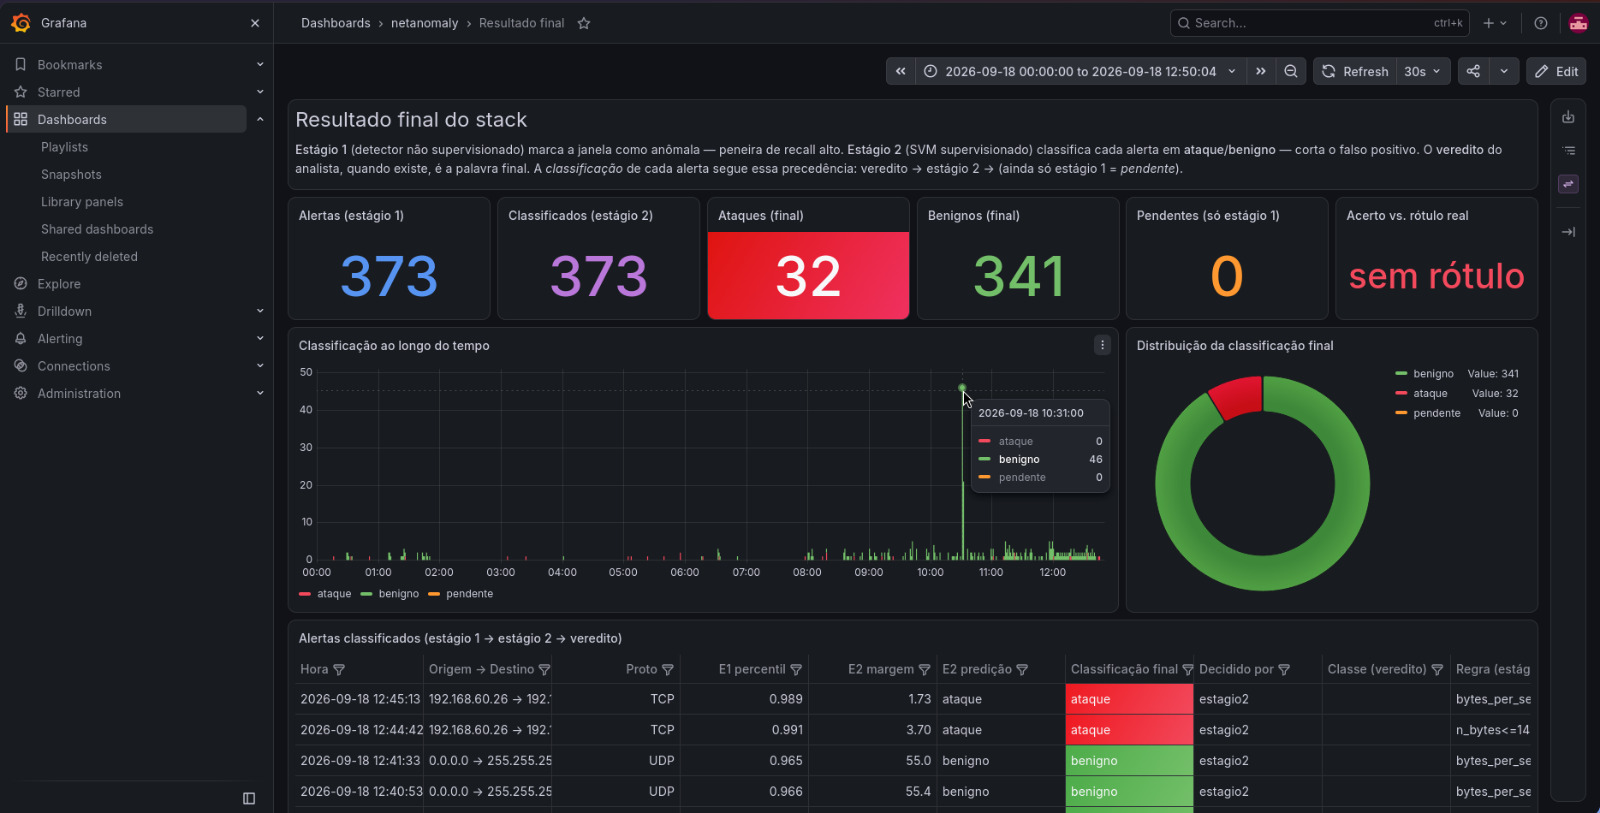
\includegraphics[width=\textwidth]{anomalia_benigna.jpg}
	\caption{Painel \textit{Resultado final} em 18/09/2026: pico de 46 alertas às 10h31, causado pelo reinício do modem e classificado inteiramente como benigno pelo estágio 2.}
	\label{fig:anomalia_benigna}
\end{figure}
\end{strip}

O caso ilustra a função do segundo estágio. No período, o estágio 2 retirou 341 dos
373 alertas (91,4\%) do caminho do analista, que passou a revisar 32 alertas em vez
de 373. Os 32 classificados como ataque não têm veredito registrado e, por isso, não
podem ser contados como acertos ou erros. Eles vão para a fila de revisão, ordenados
pela margem do SVM.

\textbf{Caso 2 --- anomalia maligna: varredura de portas.} Em 25/11/2026, às 12h50,
foi executada a partir da rede do laboratório uma varredura \texttt{nmap} das 1.000
portas mais comuns de um \textit{host}. Entre 12h43 e 13h55, o estágio 1 gerou cerca
de 1.090 alertas, todos classificados pelo estágio 2: cerca de 1.000 como ataque e 85
como benignos (Figura \ref{fig:anomalia_maligna}). Na janela da varredura, o painel
registra cerca de 1.000 alertas de ataque e 1 benigno, o que corresponde a
aproximadamente um fluxo por porta sondada. Os 85 benignos do restante do período
são tráfego de fundo da rede, como UDP \textit{multicast} (\texttt{224.0.0.0/4}),
que a tabela do painel mostra com margem entre 6 e 16 do lado benigno.

\begin{strip}
\begin{figure}[H]
	\centering
	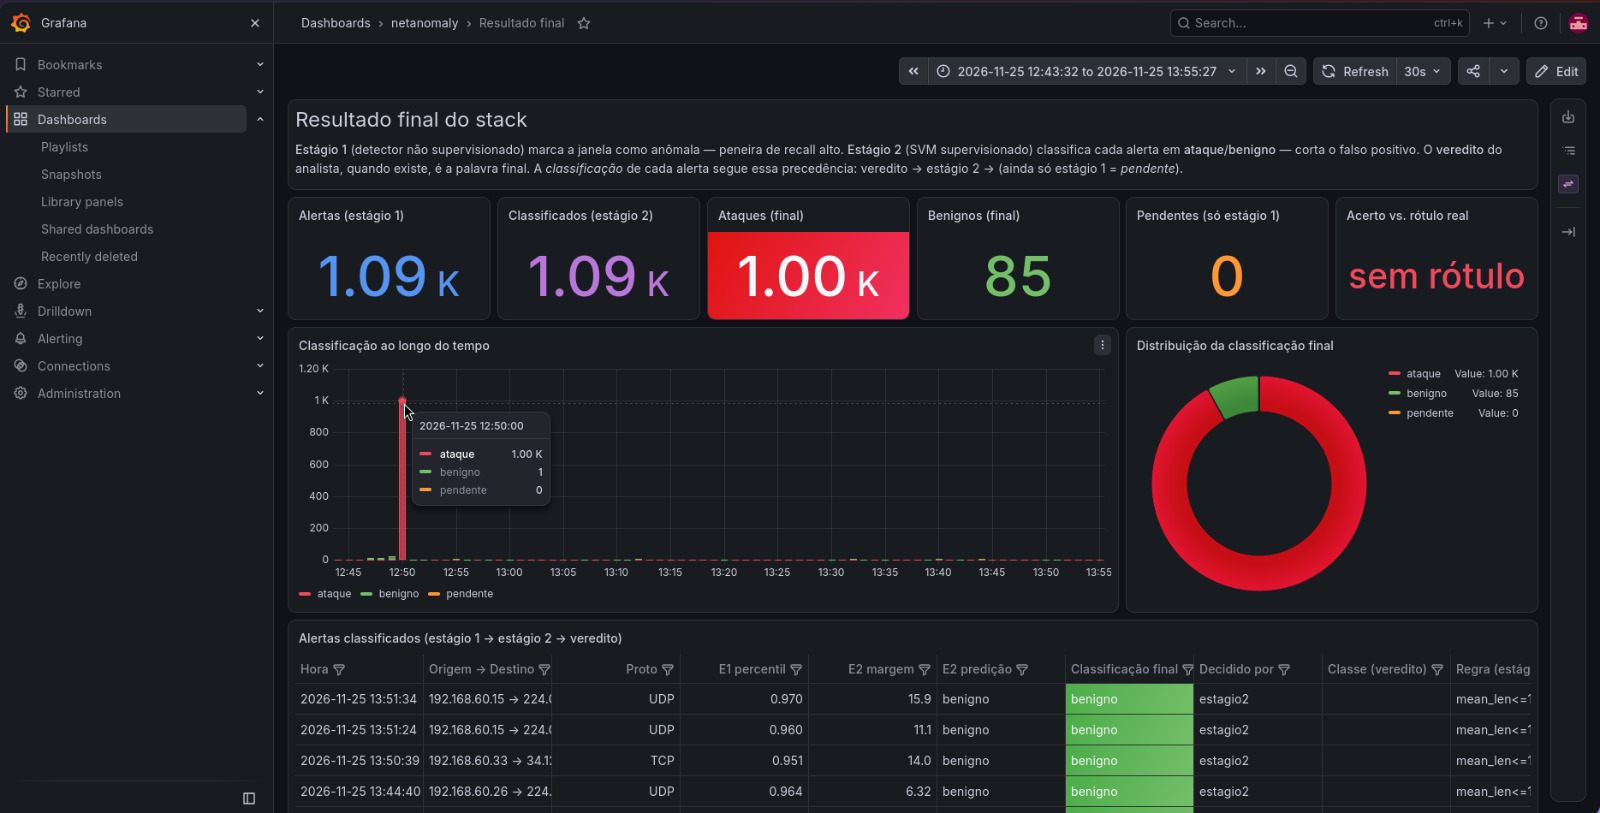
\includegraphics[width=\textwidth]{anomalia_maligna.jpg}
	\caption{Painel \textit{Resultado final} em 25/11/2026: varredura \texttt{nmap} de 1.000 portas às 12h50, com cerca de 1.000 alertas classificados como ataque pelo estágio 2.}
	\label{fig:anomalia_maligna}
\end{figure}
\end{strip}

A varredura é o contraponto do resultado do \textit{golden set}. Cada sonda gera um
fluxo curto, tipicamente de um ou dois pacotes com \texttt{SYN} sem resposta ou
respondido com \texttt{RST}, de um tipo raro no tráfego normal. Ao contrário do ataque volumoso e
homogêneo do \textit{golden set}, esses fluxos são isoláveis, e o estágio 1 os marca
como alerta. O estágio 2 confirma a classificação. O alerta aparece na mesma janela
da varredura, já que o analisador ao vivo trabalha em janelas de 10~s.

Os dois casos mostram a cascata funcionando como projetada: o estágio 1 trata como
anomalia tudo o que é raro, seja malicioso ou não, e o estágio 2 separa o reinício
do modem da varredura. A Tabela \ref{tab:casos} resume os dois cenários.

\begin{table}[H]
	\centering
	\footnotesize
	\setlength{\tabcolsep}{3pt}
	\begin{tabularx}{\columnwidth}{l X X}
		\toprule
		 & \textbf{Reinício do modem} & \textbf{Varredura \texttt{nmap}} \\
		\midrule
		Natureza          & Benigna, incomum          & Maliciosa, deliberada \\
		Alertas (estágio 1)& 373 (46 no pico)         & $\approx$1.090 ($\approx$1.000 no pico) \\
		Ataque (estágio 2) & 32 (0 no pico)           & $\approx$1.000 \\
		Benigno (estágio 2)& 341 (46 no pico)         & 85 (1 no pico) \\
		Resultado         & Suprimido antes do analista & Encaminhado como ataque \\
		\bottomrule
	\end{tabularx}
	\caption{Comparação dos dois estudos de caso em tráfego real.}
	\label{tab:casos}
\end{table}

\section{Conclusão}
Este trabalho apresentou uma análise exploratória e experimental de técnicas de \textit{Machine Learning} aplicadas a Sistemas de Detecção de Intrusões em Redes ($NIDS$), utilizando como referência o conjunto de dados $NSL-KDD$. Diante do desafio imposto pelo crescimento expressivo do tráfego de rede e pela sofisticação das ameaças cibernéticas contemporâneas, a pesquisa atingiu seus objetivos gerais ao mapear a eficácia de tratamentos computacionais e algorítmicos voltados à segurança da informação.

As etapas metodológicas executadas evidenciaram que o pré-processamento rigoroso — envolvendo desde a conversão de atributos categóricos via \textit{Label Encoding} até o agrupamento de ataques em macrocategorias — constitui um pilar fundamental para garantir a estabilidade e a interpretabilidade dos classificadores. Além disso, a aplicação combinada da Análise de Componentes Principais ($PCA$) e a seleção de características via $Decision Tree$ comprovaram que a redução de dimensionalidade é viável e necessária, mitigando o alto custo computacional sem comprometer a acurácia global da detecção. Os experimentos demonstraram, em alinhamento com a literatura estudada, que conjuntos reduzidos de atributos altamente discriminantes são capazes de otimizar a latência operacional de sistemas preditivos.

Por fim, os resultados obtidos demonstram o potencial da utilização de técnicas de \textit{Machine Learning} aplicadas à detecção de intrusões, especialmente quando associadas a estratégias adequadas de seleção e redução de atributos. Como trabalhos futuros, pretende-se realizar a implementação de melhorias no modelo selecionado, visando ampliar sua capacidade de generalização, eficiência e robustez frente a diferentes cenários de ataques. Além disso, busca-se aplicar as técnicas desenvolvidas na construção de um protótipo funcional de Sistema de Detecção de Intrusões em tempo real, permitindo validar, em um ambiente mais próximo do real, a viabilidade prática, o desempenho operacional e a capacidade de resposta da solução proposta diante de tráfegos e ameaças reais de rede.

% Como limitações identificadas no estágio atual do projeto, destaca-se o desbalanceamento intrínseco das classes minoritárias de ataques (como U2R e R2L) presente na base histórica utilizada, um fator que exige técnicas avançadas de reamostragem para não enviesar os modelos de aprendizado supervisionado. 

\subsection{Cronograma}

\begin{enumerate}
	\item \textbf{Definição do Tema de Pesquisa:} Realização de estudos introdutórios sobre a área de Segurança da Informação, com foco em $IDS$ e aplicação de técnicas de Machine Learning na detecção de ameaças cibernéticas.
	\item \textbf{Levantamento de Referências Bibliográficas:} Levantamento de trabalhos sobre detecção de intrusões, pré-processamento e algoritmos de \textit{Machine Learning}.
	\item \textbf{Desenvolvimento do MVP1:} Aplicação prática dos modelos utilizando a base NSL-KDD, envolvendo etapas de pré-processamento de dados, treinamento e avaliação de algoritmos supervisionados, com análise de métricas de desempenho para definição do modelo mais adequado, além da consolidação da fundamentação teórica e dos estudos realizados ao longo da pesquisa.
	\item \textbf{Apresentação do Trabalho de Conclusão de Curso:} Apresentação formal do projeto desenvolvido, abordando fundamentação teórica, metodologia aplicada, desenvolvimento do MVP, resultados alcançados e considerações finais do trabalho.
	\item \textbf{Desenvolvimento do MVP2:} Implementação de melhorias do pipeline em dois estágios, ciclo de vida, persistência, contêineres e painéis.
	\item \textbf{Entrega do Trabalho de Conclusão de Curso:} Submissão do relatório final do projeto, contendo a descrição detalhada de todas as etapas realizadas, análises dos resultados obtidos e conclusões derivadas da pesquisa.
\end{enumerate}

\begin{strip}
\centering
\footnotesize
\renewcommand{\arraystretch}{0.9}
\setlength{\tabcolsep}{2pt}

\begin{tabular}{|p{2.5cm}|*{12}{c|}}
\hline

\multirow{2}{*}{\textbf{Item}} 
& \multicolumn{12}{c|}{\textbf{2026}} \\ \cline{2-13}

& Jan & Fev & Mar & Abr & Mai & Jun & Jul & Ago & Set & Out & Nov & Dez \\
\hline

Definição do tema & X & X &  &  &  &  &  &  &  &  &  &  \\
\hline

Revisão bibliográfica &  & X & X & X &  &  &  &  &  &  &  &  \\
\hline

Desenvolvimento MVP1 &  &  &  & X & X &  &  &  &  &  &  &  \\
\hline

Apresentação do TCC &  &  &  &   &   & X &  &  &  &  &  &  \\
\hline

Desenvolvimento MVP2 &  &  &  &   &   &  & X & X & X & X & X &  \\
\hline

Entrega do TCC &  &  &  &   &   &  &  &  &  &  &  & X \\
\hline

\end{tabular}
\captionof{table}{Cronograma do projeto}
\end{strip}


\section{Referências}
\printbibliography[heading=none]

\section{Agradecimentos}
Agradecemos, primeiramente, às nossas famílias, pelo apoio incondicional,
incentivo constante e compreensão ao longo de toda a nossa trajetória 
acadêmica. Sem esse suporte, a realização deste trabalho não seria
possível.

Como inspiração para seguir em frente diante dos desafios, destacamos 
a frase de Walt Disney: “Todos os seus sonhos podem se tornar realidade 
se você tiver a coragem para persegui-los”.

\section{Anexos}
\begin{table*}[htbp]
\centering
\fontsize{10}{12}\selectfont
\renewcommand{\arraystretch}{1.2}

\begin{adjustbox}{width=\textwidth}
\begin{tabular}{p{4cm} c p{3cm} c p{3cm} c c c p{4cm} c p{4cm}}
\toprule
Título & Citações & Autor & Ano & Tipo & HIDS/NIDS & Sig. & Técnica & Técnica Utilizada & Desempenho & Base \\
\midrule

\cite{patrick2022study} & 172 & Vanin et al. & 2022 & Revisão & Ambos & Ambos & Ambos & CNN, DNN, SVM, Ensembles & 99,24\% (Acurácia) & KDD99, NSL-KDD, UNSW-NB15, CICIDS2017 \\

\cite{Thakkar2021Survey} & 459 & Thakkar \& Lohiya & 2022 & Pesquisa/Revisão & NIDS & Ambos & Ambos & ML, DL e SWEVO & 95,5\% (Acurácia) & KDD99, NSL-KDD, CICIDS2017 \\

\cite{Abdulganiyu2023Systematic} & 330 & Abdulganiyu et al. & 2022 & SLR & NIDS & Ambos + Híbrido & Sup. & CNN, ANN, RF, SVM, DT & CNN+AE (~100\%) & KDD99, NSL-KDD, UNSW-NB15 \\

\cite{Depren2005Intelligent} & 803 & Depren et al. & 2005 & Proposta & NIDS & Híbrido & Ambos & SOM (N. Sup.) e J.48 (Sup.) & 99,84\% (Uso Indevido) & KDD Cup 99 \\

\cite{Xianwei2019Adaptive} & 696 & Gao et al. & 2019 & Proposta & NIDS & Anomalia & Supervisionada & Ensemble (DT, RF, KNN, DNN) & 85,2\% (Acurácia) & NSL-KDD \\

\cite{felix2014analysis} & 293 & Iglesias \& Zseby & 2015 & Análise & NIDS & Anomalia & Supervisionada & DTC, kNN, NB, ANN, SVM & 78,68\% (Acurácia) & NSL-KDD \\

\cite{zehedi2023comparative} & 319 & Azam et al. & 2023 & Revisão & NIDS & Híbrido & Supervisionada & DT (C4.5, ID3, CART) & 97,36\% (Acurácia) & NSL-KDD, ADFA, KDD99 \\

\cite{diptiben2022cyber} & 253 & Ghelani et al. & 2022 & Visão Geral & NIDS/Ciberseg. & Geral & Plataforma IA & Geral ML/DL & Qualitativo & Bibliográfica \\

\cite{wasyhun2023cyber} & 466 & Admass et al. & 2024 & Revisão & Geral & Geral & Ambos & ML/DL & Síntese de Estado da Arte & EHR (Tempo Real) \\

\cite{Khraisat2019Hybrid} & 256 & Khraisat et al. & 2020 & Proposta & Ambos & Híbrido & Supervisionada & Stacking (C5.0 + One-Class SVM) & 97,04\% (ADFA) & NSL-KDD, ADFA \\

\cite{Jabez2015Intrusion} & 365 & Jabez \& Muthukumar & 2015 & Proposta & NIDS & Anomalia & Não Sup. & NOF (Outlier Detection) & Tempo de CPU superior & KDD Cup 99 \\

\cite{Othman2018Intrusion} & 305 & Othman et al. & 2018 & Proposta & NIDS & Anomalia & Supervisionada & SVMWithSGD (Spark) & 99,55\% (AUROC) & KDD Cup 99 \\

\cite{Liao2013Intrusion} & 2463 & Liao et al. & 2013 & Revisão & Vários & AD, SD, SPA & Vários & Bayes, Game Theory, Data Mining & Alta Acurácia (em SVM/DM) & KDD Cup 99 \\

\cite{Kazi2019network} & 327 & Taher et al. & 2019 & Estudo de Caso & NIDS & Anomalia & Supervisionada & SVM e ANN & 94,02\% (Acurácia) & NSL-KDD \\

\cite{Saranya2020Performance} & 555 & Saranya et al. & 2020 & Revisão/Prop. & Ambos & Ambos + Híb. & Supervisionada & LDA, CART, RF & 99,81\% (Acurácia) & KDD-CUP \\

\cite{Shah2018Performance} & 332 & Shah \& Issac & 2018 & Estudo Comp. & NIDS (Snort) & Híbrido & Supervisionada & SVM, DT, Fuzzy, Naive Bayes & SVM superior & Snort logs, DARPA, NSL-KDD \\

\cite{Belavagi2016Performance} & 482 & Belavagi \& Muniyal & 2016 & Estudo de Caso & NIDS & Anomalia/Uso Ind. & Supervisionada & LR, SVM, GNB, RF & 99\% (Acurácia) & NSL-KDD \\

\cite{Rathore2016RealTime} & 147 & Rathore et al. & 2017 & Proposta & NIDS & Anomalia & Supervisionada & REPTree, J48, SVM, NB & 99\% (Taxa Ver. Pos.) & DARPA, KDD99, NSL-KDD \\

\cite{Khraisat2019Survey} & 256 & Khraisat et al. & 2020 & Proposta & Ambos & Híbrido & Supervisionada & Stacking (C5.0 + One-Class SVM) & 97,04\% (ADFA) & NSL-KDD, ADFA \\

\cite{solane2015using} & 175 & Duque \& Omar & 2015 & Proposta & NIDS context & Anomalia & Não Sup. & K-means (Clustering) & 81,61\% (Eficiência) & NSL-KDD \\

\cite{emad2022intrusion} & 175 & Abdallah et al. & 2022 & Pesquisa & NIDS focus & Anomalia/Uso Ind. & Supervisionada & RF, SVM, LR, GNB, J48, DNN & 99,9\% (Acurácia em RF) & KDD99, NSL-KDD, CICIDS2017 \\

\cite{James2023Introduction} & 1879 & James et al. & 2023 & Estudo Didático & Não se aplica & Não se aplica & Ambos & LR, DT, SVM, RF, KNN, PCA, K-means e outros & Não se aplica & Bases didáticas \\

\cite{IBM2026Supervised} & Não se aplica & Belcic et al. & 2026 & Estudo Didático & Não se aplica & Não se aplica & Ambos & LR, DT, SVM, RF, KNN e outros & Não se aplica & Bases didáticas \\

\cite{scikit2026learn} & Não se aplica & Scikit-Learn & 2026 & Estudo Didático & Não se aplica & Não se aplica & Ambos & LR, DT, SVM, RF, KNN e outros & Não se aplica & Bases didáticas \\

\cite{Merkel2014Docker} & 7419 & Merkel \& Dirk & 2014 & Visão geral / Estudo técnico & Não se aplica & Não se aplica & Não se aplica & Não se aplica & Não se aplica & Não se aplica \\

\cite{Tony2008Isolation} & 13632 & F. T. Liu \& K. M. Ting \& Z.-H. Zhou, & 2008 & Proposta / Pesquisa experimental & Não se aplica & Anomalia & Não Supervisionada & Isolation Forest & Alta AUC e tempo de execução linear $O(n)$, superando LOF, ORCA e Random Forest em eficiência e escalabilidade & 12 bases públicas (UCI e dados sintéticos), incluindo KDDCup99 (http, smtp, forestcover, shuttle, breastw, etc.) \\

\cite{Corinna1995Support} & 90227 & Cortes \& Vapnik & 1995 & Proposta / Pesquisa teórica e experimental & Não se aplica & Não se aplica & Supervisionada & SVM e Kernel Trick & Taxas de erro altamente competitivas frente a redes neurais e classificadores da época, com forte generalização & USPS e NIST (reconhecimento óptico de dígitos manuscritos) \\

\cite{Battista2012Poisoning} & 2893 & Biggio \& Nelson \& Laskov & 2012 & Pesquisa experimental / Análise de segurança & Não se aplica & Não se aplica & Supervisionada & SVM & Demonstração de degradação severa da acurácia de teste da SVM com injeção de uma pequena fração de pontos maliciosos & Dados sintéticos 2D e subconjunto da base MNIST (classificação de dígitos) \\

\cite{Settles2009Active} & 10434 & B. Settles & 2009 & Revisão da literatura (Survey) & Não se aplica & Não se aplica & Semi-Supervisionada & Active Learning & Redução significativa no número de instâncias rotuladas necessárias para atingir acurácia equivalente ao aprendizado passivo & Não se aplica \\


\bottomrule
\end{tabular}
\end{adjustbox}

\caption{Revisão dos trabalhos utilizados como referência para o desenvolvimento do trabalho.}
\end{table*}

\end{document}
\documentclass[a4paper,10pt, twocolumn]{article}
\usepackage[a4paper,top=2cm,bottom=3cm,left=2cm,right=2cm,footskip=0.8cm]{geometry}
\cite{Jabez2015Intrusion} & 365 & Jabez \& Muthukumar & 2015 & Proposta & NIDS & Anomalia & Não Sup. & NOF (Outlier Detection) & Tempo de CPU superior & KDD Cup 99 \\

\cite{Othman2018Intrusion} & 305 & Othman et al. & 2018 & Proposta & NIDS & Anomalia & Supervisionada & SVMWithSGD (Spark) & 99,55\% (AUROC) & KDD Cup 99 \\

\cite{Liao2013Intrusion} & 2463 & Liao et al. & 2013 & Revisão & Vários & AD, SD, SPA & Vários & Bayes, Game Theory, Data Mining & Alta Acurácia (em SVM/DM) & KDD Cup 99 \\

\cite{Kazi2019network} & 327 & Taher et al. & 2019 & Estudo de Caso & NIDS & Anomalia & Supervisionada & SVM e ANN & 94,02\% (Acurácia) & NSL-KDD \\

\cite{Saranya2020Performance} & 555 & Saranya et al. & 2020 & Revisão/Prop. & Ambos & Ambos + Híb. & Supervisionada & LDA, CART, RF & 99,81\% (Acurácia) & KDD-CUP \\

\cite{Shah2018Performance} & 332 & Shah \& Issac & 2018 & Estudo Comp. & NIDS (Snort) & Híbrido & Supervisionada & SVM, DT, Fuzzy, Naive Bayes & SVM superior & Snort logs, DARPA, NSL-KDD \\

\cite{Belavagi2016Performance} & 482 & Belavagi \& Muniyal & 2016 & Estudo de Caso & NIDS & Anomalia/Uso Ind. & Supervisionada & LR, SVM, GNB, RF & 99\% (Acurácia) & NSL-KDD \\

\cite{Rathore2016RealTime} & 147 & Rathore et al. & 2017 & Proposta & NIDS & Anomalia & Supervisionada & REPTree, J48, SVM, NB & > 99\% (Taxa Ver. Pos.) & DARPA, KDD99, NSL-KDD \\

\cite{Khraisat2019Survey} & 256 & Khraisat et al. & 2020 & Proposta & Ambos & Híbrido & Supervisionada & Stacking (C5.0 + One-Class SVM) & 97,04\% (ADFA) & NSL-KDD, ADFA \\

\cite{solane2015using} & 175 & Duque \& Omar & 2015 & Proposta & NIDS context & Anomalia & Não Sup. & K-means (Clustering) & 81,61\% (Eficiência) & NSL-KDD \\

\cite{emad2022intrusion} & 175 & Abdallah et al. & 2022 & Pesquisa & NIDS focus & Anomalia/Uso Ind. & Supervisionada & RF, SVM, LR, GNB, J48, DNN & 99,9\% (Acurácia em RF) & KDD99, NSL-KDD, CICIDS2017 \\

\cite{James2023Introduction} & 1879 & James et al. & 2023 & Estudo Didático & Não se aplica & Não se aplica & Ambos & LR, DT, SVM, RF, KNN, PCA, K-means e outros & Não se aplica & Bases didáticas \\


\bottomrule
\end{tabular}
\end{adjustbox}

\caption{Revisão dos trabalhos sobre IDS}
\end{table*}

\section{Agradecimentos}
Agradecemos, primeiramente, às nossas famílias, pelo apoio incondicional,
incentivo constante e compreensão ao longo de toda a nossa trajetória 
acadêmica. Sem esse suporte, a realização deste trabalho não seria
possível.

Como inspiração para seguir em frente diante dos desafios, destacamos 
a frase de Walt Disney: “Todos os seus sonhos podem se tornar realidade 
se você tiver a coragem para persegui-los”.

\end{document}
